%%%%%%%%%%%%%%%%%%%%%%%%%%%%%%%%%%%%%%%%%%%%%%%%%%%%%%%%%%%%%%%%%%%%%%%%%%%%%%
%
% MASTER FILE START
%
%%%%%%%%%%%%%%%%%%%%%%%%%%%%%%%%%%%%%%%%%%%%%%%%%%%%%%%%%%%%%%%%%%%%%%%%%%%%%%

\RequirePackage{ifpdf}
\ifpdf
  \documentclass[ignoreframetext,mathserif]{beamer}
\else
  \documentclass[ignoreframetext,dvips,trans]{beamer}
\fi

%%%%%%%%%%%%%%%%%%%%%%%%%%%%%%%%%%%%%%%%%%%%%%%%%%%%%%%%%%%%%%%%%%%%%%%%%%%%%%
%
% PACKAGES
%
%%%%%%%%%%%%%%%%%%%%%%%%%%%%%%%%%%%%%%%%%%%%%%%%%%%%%%%%%%%%%%%%%%%%%%%%%%%%%%
\usepackage{etex}
% \usepackage{umoline}
\usepackage[]{fontenc}         % select new font encodings
\usepackage[latin1]{inputenc}  % select input encoding
\usepackage{fancybox}          % nice boxes
\usepackage{ifpdf}             % using the ifpdf conditional
\usepackage{alltt}             % use tex-environments inside verbatim
\usepackage{epsfig}            % another way to include eps-figures
%\usepackage{epic,eepic}        % extended picture environments
\usepackage{graphicx,color}    % support for including graphics
%\usepackage{latexsym}          % symbols
\usepackage{xspace}            % intelligent space after macros
\usepackage{url}               % url typeset correctly
\usepackage{epstopdf}          % on-the-fly conversion of eps to pdf when needed
\usepackage{booktabs}
\usepackage{multirow}
\usepackage{bussproofs}
\usepackage{amssymb}
\usepackage{amsmath}
\usepackage{stmaryrd}
\usepackage{tikz}
\usetikzlibrary{arrows}
\DeclareGraphicsRule{.pdftex}{pdf}{.pdftex}{}

\usepackage{amstext,amssymb,amsbsy}
\usepackage{amsmath}
\usepackage{pifont}
\usepackage{mathrsfs}

\mode<article>
{
\usepackage{fullpage}
}

% \newcommand{\sa}[0]{\textrm{a}}
% \newcommand{\se}[0]{\textrm{e}}
% \newcommand{\si}[0]{\textrm{i}}
% \newcommand{\so}[0]{\textrm{o}}
% \renewcommand{\sa}[0]{\mbox{$\mathrm{a}$}}
% \renewcommand{\se}[0]{\mbox{$\mathrm{e}$}}
% \renewcommand{\si}[0]{\mbox{$\mathrm{i}$}}
% \renewcommand{\so}[0]{\mbox{$\mathrm{o}$}}
%
 \newcommand{\nafo}[0]{\mathit{not}}
 \renewcommand{\nafo}[0]{\mathrm{not}}
 %\newcommand{\naf}[0]{\nafo\;}
% % \renewcommand{\naf}{\ensuremath{\mathrm{not}\;}}
% \newcommand{\U}{{\cal U}}
% \newcommand{\Set}{{\mathcal S}}
% \newcommand{\LA}{\mathcal{P}_A}
% \newcommand{\LU}{\mathcal{P}_{\U}}
% \newcommand{\AS}[1]{\mathit{AS}(#1)}
% \newcommand{\SM}{\mathcal{AS}}
% \renewcommand{\L}{{\cal L}}
%
% \newcommand{\meta}{\preceq}
% \renewcommand{\meta}{\odot}
% \newcommand{\revmeta}{\succeq}
% \newcommand{\sub}[1]{{\subseteq_{#1}}}
% \newcommand{\eqa}[1]{=_{#1}}
% \newcommand{\mould}[1]{\mu_{#1}}
 \newcommand{\wed}[1]{\omega_{#1}}
% \newcommand{\lpcl}[0]{{\cal C}}
% \newcommand{\C}[0]{\lpcl}
% \renewcommand{\P}[0]{{\cal P}}
 \renewcommand{\S}[0]{{\mathit{S}}}
% \newcommand{\R}{\rho}
 \newcommand{\PiP}[1]{{\Pi}_{#1}^{P}}

\newcommand{\kato}[0]{\texttt{Kato}}
\newcommand{\dlv}{\texttt{DLV}}
\newcommand{\clasp}{\texttt{Clasp}}
\newcommand{\smodels}{\texttt{SModels}}
\newcommand{\match}{\texttt{Match}}
\newcommand{\lparse}{\texttt{LParse}}
\newcommand{\gringo}{\texttt{Gringo}}

\newcommand{\lit}[1]{\mathit{lit}(#1)}
\newcommand{\litH}[1]{\mathit{lit_H}(#1)}
\newcommand{\litB}[1]{\mathit{lit_B}(#1)}


%%%%%%%%%%%%%%%%%%%%%%%%%%%%%%%%%%%%%%%%%%%%%%%%%%%%%%%%%%%%%%%5
\renewcommand{\b}[0]{\bigskip}
\newcommand{\gdw}[0]{~$\Longleftrightarrow$~}
\newcommand{\commadots}[0]{,\ldots ,}
\newcommand{\magenta}[1]{\textcolor{magenta}{#1}}
%\newcommand{\blue}[1]{\textcolor{blue}{#1}}
\newcommand{\blue}[1]{\textcolor{red!30!green!30!blue!100}{#1}}
\renewcommand{\magenta}[1]{\textcolor{red}{#1}}
\newcommand{\Th}[1]{\mathit{Th}(#1)}
\newcommand{\hence}{\;\dot{.\;.}\;}
\newcommand{\quantifier}{{\sf Q}}
\newcommand{\dt}{T=\langle W,D\rangle}
\newcommand{\reduct}[2]{#1^{#2}}
\newcommand{\Cn}[1]{\Th{#1}}
%%%%%%%%%%%%%%%%%%%%%%%%%%%%%%%%%%%%%%%%%%%%%%%%%%%%%%%%%%%%%%%%

\newcommand{\union}{\cup}
\newcommand{\la}{\leftarrow}
\newcommand{\enc}[1]{\mathcal{T}[#1]}
\newcommand{\eqcheck}{\texttt{cc}$\top$}


%%%%%%%%%%%%%%%%%%%%%%%%%%%%%%%%%%%%%%%%%%%%%%%%%%%%%%%%%%%%%%%%%%%%%%%%%%%%%%
%
% CUSTOM BEAMER STYLE
%
%%%%%%%%%%%%%%%%%%%%%%%%%%%%%%%%%%%%%%%%%%%%%%%%%%%%%%%%%%%%%%%%%%%%%%%%%%%%%%

%\useoutertheme{infolines}

\setbeamersize{text margin left=0.5cm}
\setbeamersize{text margin right=0.5cm}
\setbeamercovered{invisible}

%\definecolor{orange}{cmyk}{0,0.61,0.87,0}

%\newcommand{\myhead}[1]{\hskip0.3cm\raisebox{-0.2cm}[.5cm][.5cm]{\scriptsize
%  \ifpdf\includegraphics[width=1cm]{figures/logo-basic.pdf}\else\epsfig{file=figures/logo-basic.eps,width=1cm}\fi}\phantom{Text}
%  \hfill{\scriptsize {\usebeamercolor[fg]{frametitle} #1}}\hskip0.3cm\strut}

\newcommand{\myfoot}{\hskip0.3cm\raisebox{-0.2cm}[.5cm][.5cm]{\scriptsize
  \ifpdf\includegraphics[width=1cm]{figures/logo-basic.pdf}\else\epsfig{file=figures/logo-basic.eps,width=1cm}\fi}\phantom{Text}\hfill\raisebox{-.07cm}{\scriptsize\insertframenumber}\hskip0.3cm\strut}
%\setbeamertemplate{headline}[text line]{\myhead{\insertsubsection}}

\newcommand{\myfootalt}{%
       \leavevmode%
       \hbox{\begin{beamercolorbox}[wd=.5\paperwidth]{navigation symbols}%
%           \includegraphics[width=1cm]{figures/logo-basic}
\nop{           \insertslidenavigationsymbol
           \insertframenavigationsymbol
           \insertsubsectionnavigationsymbol
           \insertsectionnavigationsymbol
           \insertdocnavigationsymbol
           \insertbackfindforwardnavigationsymbol
}
         \end{beamercolorbox}%
         \begin{beamercolorbox}[wd=.5\paperwidth,dp=1ex,rightskip=1ex plus1fil]{title in head/foot}%\newcommand{\antiseq}{\dashv}%{\not\vdash}
\newcommand{\seq}{\vdash}
\def\fCenter{{\mbox{$~\antiseq~$}}}



           \hfill
           \insertframenumber /\inserttotalframenumber
         \end{beamercolorbox}}%
       \vskip0pt%
     }

\setbeamertemplate{navigation symbols}{}
\setbeamertemplate{footline}{\myfootalt}

\setbeamertemplate{frametitle}{
\begin{centering}
    \insertframetitle\par
\end{centering}
}

\setbeamertemplate{part page}{
\frametitle{\vspace{4ex}\inserttitle\\[2ex]\insertpart}
\begin{centering}
\insertauthor\par
\end{centering}
\begin{centering}
\vspace*{3ex}{\scriptsize \insertinstitute}\par
\end{centering}
\vspace*{4ex}\par
\begin{centering}
\insertdate
\end{centering}
}

\AtBeginPart{
\frame[plain]{\partpage}
\addtocounter{framenumber}{-1}
}

\mode<presentation>
{
\newtheorem{mybox}[]{}
}

\mode<article>
{
\newcommand{\mybox}{}
}


%\newcommand{\blue}[1]{\textcolor{blue}{#1}}
%\newcommand{\blue}[1]{\textcolor{red!30!green!30!blue!90}{#1}}

\newcommand{\red}[1]{\textcolor{red}{#1}}
\ifpdf
  \newcommand{\yellow}[1]{\textcolor{orange}{#1}}
\else
  \newcommand{\yellow}[1]{\blue{#1}}
\fi
\newcommand{\green}[1]{\textcolor{green}{#1}}
\newcommand{\white}[1]{\textcolor{white}{#1}}
\newcommand{\black}[1]{\textcolor{black}{#1}}

\mode<handout|trans|article>
{
\renewcommand{\yellow}[1]{\blue{#1}}
}


\newcommand{\bluearrow}{\blue{\Pisymbol{pzd}{228}}}
\newcommand{\blueresarrow}{\large\blue{\Pisymbol{pzd}{229}}}
\newcommand{\greenarrow}{\green{\Pisymbol{pzd}{228}}}
\newcommand{\greenresarrow}{\large\green{\Pisymbol{pzd}{229}}}
\newcommand{\redarrow}{\red{\Pisymbol{pzd}{228}}}
\newcommand{\redresarrow}{\large\red{\Pisymbol{pzd}{229}}}
\newcommand{\yellowarrow}{\yellow{\Pisymbol{pzd}{228}}}
\newcommand{\yellowresarrow}{\large\yellow{\Pisymbol{pzd}{229}}}

\newcommand{\cemph}[1]{\yellow {\emph{#1}}}
%\newcommand{\myitem}{\item[\bluearrow]}
\newcommand{\myitem}{\item[\Pisymbol{pzd}{228}]}
\newcommand{\mi}{\myitem}
%\newcommand{\bitem}{\item[\blue {\textbf{--}}]}
\newcommand{\bitem}{\item[{\textbf{--}}]}
%\newcommand{\resitem}{\item[\blueresarrow]}
\newcommand{\resitem}{\item[\large{\Pisymbol{pzd}{229}}]}
\newcommand{\h}{\yellow {$\Longrightarrow$}}

\newcommand{\itarrow}{\yellow{\Pisymbol{pzd}{229}}}
\newcommand{\ithook}{\yellow{\Pisymbol{pzd}{52}}}
\newcommand{\itcross}{\yellow{\Pisymbol{pzd}{56}}}
\newcommand{\ithand}{\yellow{\Pisymbol{pzd}{43}}}


\setbeamertemplate{itemize item}{\Pisymbol{pzd}{228}}
\setbeamertemplate{itemize subitem}{{$\bullet$}}
\setbeamertemplate{itemize subsubitem}{\textbf{--}}

%
% Use equal font size at all levels (of itemization and enumeration)
%
\setbeamerfont{itemize/enumerate subbody}{size=\normalsize}
\setbeamerfont{itemize/enumerate subsubbody}{size=\normalsize}
\setbeamerfont{itemize subitem}{size=\normalsize}
\setbeamerfont{itemize subsubitem}{size=\normalsize}
\setbeamerfont{enumerate subitem}{size=\normalsize}
\setbeamerfont{enumerate subsubitem}{size=\normalsize}


\mode<article>
{
\renewcommand{\labelitemi}{\blue{\Pisymbol{pzd}{228}}}
\renewcommand{\labelitemii}{\blue{$\bullet$}}
\renewcommand{\labelitemiii}{\blue{\textbf{--}}}
}

\mode<handout|trans>
{
\beamertemplatenavigationsymbolsempty
}

\ifpdf
\else
  \beamertemplatenavigationsymbolsempty
\fi


%%%%%%%%%%%%%%%%%%%%%%%%%%%%%%%%%%%%%%%%%%%%%%%%%%%%%%%%%%%%%%%%%%%%%%%%%%%%%%
%
% MACROS
%
%%%%%%%%%%%%%%%%%%%%%%%%%%%%%%%%%%%%%%%%%%%%%%%%%%%%%%%%%%%%%%%%%%%%%%%%%%%%%%

%\def\AND     { \,\wedge\,                 }
%\def\OR      { \,\vee\,                   }
%\def\XOR     { \,\stackrel{.}{\vee}\,     }
%\def\IMPLIES { \,\supset\,                }
%\def\IMPL    { \,\supset\,                }
%\def\IF      { \,\leftarrow\,             }
%\def\IFF     { \,\equiv\,         }
%\def\IFFdef  { \,\stackrel{\rm def}{\longleftrightarrow}\, }

\newcommand{\iec}[0]{i.e.,\ }
\newcommand{\egc}[0]{e.g.,\ }
\newcommand{\ra}[0]{\rightarrow}
\newcommand{\Ra}[0]{$\Rightarrow$\ }
\newcommand{\bi}[0]{\begin{itemize}\itemsep=+.5ex}
\newcommand{\ei}[0]{\end{itemize}}
\newcommand{\bdescr}[0]{\begin{description}}
\newcommand{\edescr}[0]{\end{description}}
\newcommand{\be}[0]{\begin{enumerate}\itemsep=+.5ex}
\newcommand{\ee}[0]{\end{enumerate}}

\newcommand\nop[1]{}


%%%%%%%%%%%%%% SPACING COMMANDS

\newcommand{\nbls}{\vspace*{-1\baselineskip}}
\newcommand{\hnbls}{\vspace*{-.5\baselineskip}}
\newcommand{\tnbls}{\vspace*{-.33\baselineskip}}
\newcommand{\qnbls}{\vspace*{-.25\baselineskip}}

\newcommand{\bls}{\vspace*{1\baselineskip}}
\newcommand{\hbls}{\vspace*{.5\baselineskip}}
\newcommand{\tbls}{\vspace*{.33\baselineskip}}
\newcommand{\qbls}{\vspace*{.25\baselineskip}}

\newcommand{\bs}{\bigskip}
\newcommand{\ms}{\medskip}
%\newcommand{\b}{\bigskip}
\newcommand{\m}{\medskip}
\newcommand{\s}{\smallskip}
\newcommand{\sm}{\smallskip}

\tikzset{
  treenode/.style = {align=center, inner sep=0pt, text centered, circle, draw=black},
  arn_n/.style = {treenode, circle, draw=black, text width=1.5em}
}

\newcommand{\shortasp}[1]{\mathtt {#1} }

\newenvironment{aspenv}{\begin{ttfamily}\begin{tabular}{l}}{\end{tabular} \end{ttfamily}}
\newenvironment{asparray}{\begin{eqnarray}}{\end{eqnarray}\noindent}
\newenvironment{asparray*}{\begin{eqnarray*}}{\end{eqnarray*}}%

% not in math env
\newcommand{\asp}[1]{\noindent\ensuremath{\shortasp{#1}}}
\newcommand{\aspsub}[1]{\noindent\\\ensuremath{\ \ \ x\shortasp{#1}}}

\newcommand{\naf}[1]{\mathrm{not}\ #1}

\newcommand{\head}[1]{\mathit{H}({#1})}
\newcommand{\posbody}[1]{\mathit{B^{+}}({#1})}
\newcommand{\negbody}[1]{\mathit{B^{-}}({#1})}
\newcommand{\body}[1]{\mathit{B}({#1})}

\newcommand{\wrt}{w.r.t.}

\newcommand{\inp}[1]{\mathrm{I}_{#1}}
\newcommand{\out}[1]{\mathrm{O}_{#1}}
%%%%%%%%%%%%%%%%%%%%%%%%%%%%%%%%%%%%%%%%%%%%%

%%%%%%%%%%%%%%%%%%%%%%%%%%%%%%%%%%%%%%%%

\def\implLeftA{(\IMPL l)_{1}}
\def\implLeftB{(\IMPL l)_{2}}
\def\implRight{(\IMPL r)}

\def\conjLeft{(\AND\, l)}
\def\confRightA{(\AND\, r)_{1}}
\def\confRightB{(\AND\, r)_{2}}

\def\disjLeftA{(\OR\, l)_{1}}
\def\disjLeftB{(\OR\, l)_{2}}
\def\disjRight{(\OR\, r)}

%%%%%%%%%%%%%%%%%%%%%%%

\def\negNegLeft{(\NEG\NEG\, l)}
\def\negNegRight{(\NEG\NEG\, r)}

\def\negConjLeftA{(\NEG\!\AND l)_{1}}
\def\negConjLeftB{(\NEG\!\AND l)_{2}}
\def\negConjRight{(\NEG\!\AND r)}

\def\negDisjLeft{(\NEG\!\OR l)}
\def\negDisjRightA{(\NEG\!\OR r)_{1}}
\def\negDisjRightB{(\NEG\!\OR r)_{2}}

\def\negImplLeft{(\NEG\!\IMPL l)}
\def\negImplRightA{(\NEG\!\IMPL r)_{1}}
\def\negImplRightB{(\NEG\!\IMPL r)_{2}}

\def\NegGLeft{(\NEGg\, l)}
\def\NegGRight{(\NEGg\, r)}

\def\ImplGLeftA{(\IMPLg\, l)_{1}}
\def\ImplGLeftB{(\IMPLg\, l)_{2}}
\def\ImplGLeftC{(\IMPLg\, l)_{3}}
\def\ImplGRightA{(\IMPLg\, r)_{1}}
\def\ImplGRightB{(\IMPLg\, r)_{2}}

\def\NegNegGLeft{(\NEG\NEGg\, l)}
\def\NegNegGRight{(\NEG\NEGg\, r)}

\def\NegImplGLeft{(\NEG\IMPLg\, l)}
\def\NegImplGRight{(\NEG\IMPLg\, r)}

\def\NegNegGLeft{(\NEG\!\NEGg\, l)}
\def\NegNegGRight{(\NEG\!\NEGg\, r)}

\def\NegImplGLeft{(\NEG\!\IMPLg\, l)}
\def\NegImplGRightA{(\NEG\!\IMPLg\, r)_{1}}
\def\NegImplGRightB{(\NEG\!\IMPLg\, r)_{2}}

%%%%%%%%%%%%%%%%%%%%%%%%%%%%%%%%%%%%%%%%

\newcommand{\antiseq}{\dashv}%{\not\vdash}
%\newcommand{\seq}{\vdash}
\def\fCenter{{\mbox{$~\antiseq~$}}}


\newcommand{\NEG}{\neg}
\newcommand{\AND}{\wedge}
\newcommand{\OR}{\vee}
\newcommand{\IMPL}{\supset}
\newcommand{\True}{\mathbf{t}}
\newcommand{\False}{\mathbf{f}}
\newcommand{\Indet}{\mathbf{i}}
\newcommand{\CTrue}{\mathrm{T}}
\newcommand{\CFalse}{\mathrm{F}}
\newcommand{\CIndet}{\mathrm{I}}
\newcommand{\U}{\ensuremath{\mathcal{U}}\xspace}
\newcommand{\I}{\ensuremath{\mathcal{I}}}
\newcommand{\Log}{\ensuremath{\mathcal{L}}\xspace}
\renewcommand{\P}{\ensuremath{\mathcal{P}}\xspace}
\newcommand{\ASP}{\ensuremath{\mathbf{SRCP}}\xspace}
\newcommand{\ASL}{\ensuremath{\mathbf{SRCL}}\xspace}

\newcommand{\IMPLk}{\rightarrow_{K}}
\newcommand{\IMPLl}{\rightarrow_{L}}
\newcommand{\IMPLg}{\rightarrow_{G}}
\newcommand{\NEGg}{\sim\!}
%\newcommand{\naf}{\mathrm{not}}

%\newcommand{\egc}{{e.g.,\ }}
%\newcommand{\iec}{{i.e.,\ }}
%\newcommand{\respc}{resp.,\ }
%\newcommand{\wrt}{with respect to}


\renewcommand{\phi}{\varphi}
\newcommand{\uphi}{\varphi}
\newcommand{\upsi}{\psi}
\newcommand{\uGamma}{{\Gamma}}
\newcommand{\uDelta}{{\Delta}}

\newcommand{\alc}{\ensuremath{\mathcal{ALC}}}
\newcommand{\calculus}{$\mathrm{\mathbf{SC}}_{\alc}^c$}

\newcommand{\mixforall}{$($\textsc{Mix}$, \forall)$}
\newcommand{\mixexists}{$($\textsc{Mix}$, \exists)$}
\newcommand{\mix}{$($\textsc{Mix}$)$}
\newcommand{\mixtwo}{$(\mbox{\textsc{Mix}}^2)$}
\newcommand{\sqcapl}{$(\sqcap, l)$}
\newcommand{\sqcaprone}{$(\sqcap, r)_1$}
\newcommand{\sqcaprtwo}{$(\sqcap, r)_2$}
\newcommand{\sqcupr}{$(\sqcup, r)$}
\newcommand{\sqcuplone}{$(\sqcup, l)_1$}
\newcommand{\sqcupltwo}{$(\sqcup, l)_2$}
\newcommand{\botrule}{$(\bot)$}
\renewcommand{\toprule}{$(\top)$}
\newcommand{\negl}{$(\neg, l)$}
\newcommand{\negr}{$(\neg, r)$}
\newcommand{\weakleft}{\ensuremath{(w^{-1}, l)}}
\newcommand{\weakright}{\ensuremath{(w^{-1}, r)}}

\definecolor{mymagenta}{cmyk}{0,0.6,0,0.4}
\newcommand{\mat}[1]{\textcolor{mymagenta}{#1}}

\usepackage{xcolor, colortbl}

\definecolor{LightGreen}{rgb}{0.5,0.8,0.5}
\definecolor{IntenseGreen}{rgb}{0.5,1,0.5}

\definecolor{LightYellow}{rgb}{0.82,0.81,0.58}
\definecolor{IntenseYellow}{RGB}{249,240,91}

\newcommand{\tuple}[1]{\ensuremath{\langle #1 \rangle}}
\newcommand{\type}[1]{\mathtt{#1}}
\newcommand{\personality}[5]{\tuple{\type{#1},\type{#2}, \type{#3}, \type{#4}, \type{#5}}}


\tikzset{
   every overlay node/.style={
      anchor=north west,
   },
}
% Usage:
% \tikzoverlay at (-1cm,-5cm) {content};
% or
% \tikzoverlay[text width=5cm] at (-1cm,-5cm) {content};
\def\tikzoverlay{%
   \tikz[baseline,overlay]\node[every overlay node]
}%


%%%%%%%%%%%%%%%%%%%%%%%%%%%%%%%%%%%%%%%%%%%%%%%%%%%%%%%%%%%%%%%%%%%%%%%%%%%%%%
%
% DOCUMENT PROPERTIES
%
%%%%%%%%%%%%%%%%%%%%%%%%%%%%%%%%%%%%%%%%%%%%%%%%%%%%%%%%%%%%%%%%%%%%%%%%%%%%%%

\title[Design and Implementation of an Agent Architecture combining Emotions and Reasoning]{Design and Implementation of an Agent Architecture combining Emotions and Reasoning}

\author[]{%\bf
Janos Tapolczai \\[5ex]
Vienna University of Technology \\
}


\institute[]{}

\date{
14.06.2016\\[2ex]
}

\titlegraphic{}


%%%%%%%%%%%%%%%%%%%%%%%%%%%%%%%%%%%%%%%%%%%%%%%%%%%%%%%%%%%%%%%%%%%%%%%%%%%%%%
%
% DOCUMENT START
%
%%%%%%%%%%%%%%%%%%%%%%%%%%%%%%%%%%%%%%%%%%%%%%%%%%%%%%%%%%%%%%%%%%%%%%%%%%%%%%

\begin{document}
\frame[plain]{\titlepage}
\addtocounter{framenumber}{-1}
% !TEX root = aslides.tex
   
   % this prints title, author etc. info from above
   \begin{frame}{Content}
      \tableofcontents
   \end{frame}
   
   \section{Our Goal}
   
   \begin{frame}{Our Goal}
      \begin{itemize}
         \item We wanted to design an AI that combines emotions and reasoning.
         
         \medskip
         
         \item Emotions should guide the planning and serve as \cemph{cognitive shortcuts}.
         
         \medskip
         
         \item In the design, we took cues from evolutionary neurobiology, as well as from works by Marvin Minsky and Aaron Sloman.
         
         \medskip
         
         \item In particular, the following questions motivated our approach:
         
         \begin{itemize}
            \item How could brains have evolved?
            \item Could we approximate their functioning?
            \item Would the end result be useful?
         \end{itemize}
      \end{itemize}
   \end{frame}
   
   \begin{frame}{Our Goal}
      \begin{itemize}
         \item We were not interested in logic as such; fidelity to biological systems was more important.
         
         \medskip
         
         \item Aaron Sloman (quoted from the \texttt{comp.ai.philosophy} newsgroup):
         
         \begin{quote}
            It is not worth asking how to define consciousness, how to explain it, how it
            evolved, what its function is, etc. [...]\\
            Instead, we have many sub-capabilities, for which the answers are different: e.g., different kinds of perception, learning, knowledge, attention control, self-monitoring, self-control, etc.
         \end{quote}
         
      \end{itemize}
   \end{frame}
   
   \section{Methodology}
   
   \begin{frame}{Methodology}
      \begin{itemize}
         \item We implemented a \cemph{toy AI} and a 2D world.
         \item Each agent was given a certain \cemph{personality}.
         \item The only goal was survival.
         
         \vspace{1cm}
         
         \item We tested the AI's general fitness,
         \item and we compared different personalities.
      \end{itemize}
   \end{frame}
   
   \section{Design Philosophy}
   
   \begin{frame}{Design Philosophy --- Biological Considerations}
      \begin{itemize}
         \item Neurons evolved as a means of sending signals in an organism.
         \medskip
         \item Over time, neurons began to modulate the signals of other neurons.
         \medskip
         \item This was computation of a sort, but it was not \cemph{well-designed} from an engineering standpoint.
         \medskip
         \item Moreover, there was no long-term planning.
         \medskip
         \item Functionality evolved on an \emph{ad hoc} basis.
         
         \vspace{2mm}
         
         \resitem There are no well-defined components or interfaces.
         \resitem There is no calling model.\\
         \resitem Neurons just \cemph{listen in} on the activity of others.
         
         \pause
         \medskip
         \item Thus our working hypothesis: a \cemph{White-box model of cognition}.
      \end{itemize}
   \end{frame}
   
   \begin{frame}{Design Philosophy --- White-box model}
      \begin{itemize}
         \item Traditional programming languages work via \cemph{black boxes}:\\
         \vspace{2mm}
         Functions are called, but their internals are unobservable.
         \vspace{4mm}
         \item We assume that components in the brain are \cemph{white boxes}:\\
         \vspace{2mm}
         Any component can observe the activity of others.
      \end{itemize}
   \end{frame}
   
   \begin{frame}{Design Philosophy --- White-box model}
      \begin{itemize}
         \item Of course, practical considerations apply.
         \medskip
         \item We still use regular functions within components,
         \item but components can publish \cemph{messages}.
         \medskip
         \item These are stored in a central \cemph{message space}.
         \medskip
         \item Any component can read from and write into the message space.
         \vspace{8mm}
         \item Components are \cemph{loosely coupled}:
         \resitem components don't know who reads their messages;\\
         \resitem components don't know who wrote the messages.
      \end{itemize}
   \end{frame}
   
   \section{Architecture}
   
   \begin{frame}{Architecture}
      \begin{itemize}
         \item The implementation consists of a
         \begin{itemize}
            \item \cemph{world simulator} and an
            \item \cemph{agent architecture}.
         \end{itemize}
         
         \medskip
         \item Our world is a generalisation of the \cemph{Wumpus World} of Russel and Norvig (from Artificial Intelligence: A Moden Approach, p. 236).
      \end{itemize}
   \end{frame}
   
   \begin{frame}{Architecture --- World Simulator}
      \begin{center}
         \only<1>{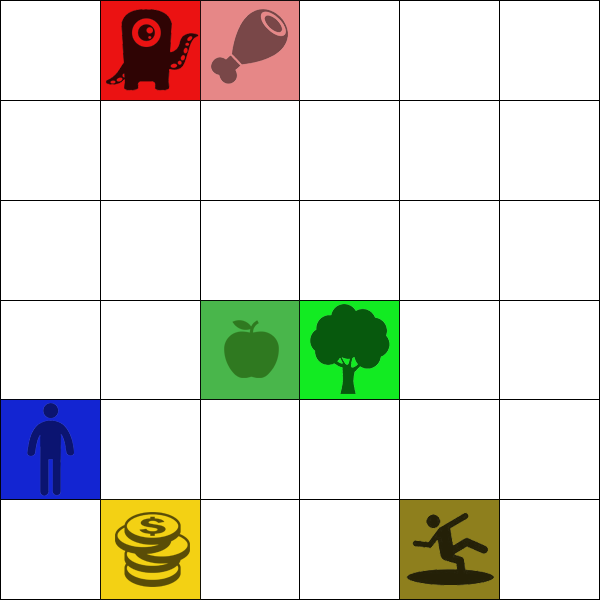
\includegraphics[width=0.65\textwidth]{map.png}}%
         \only<2>{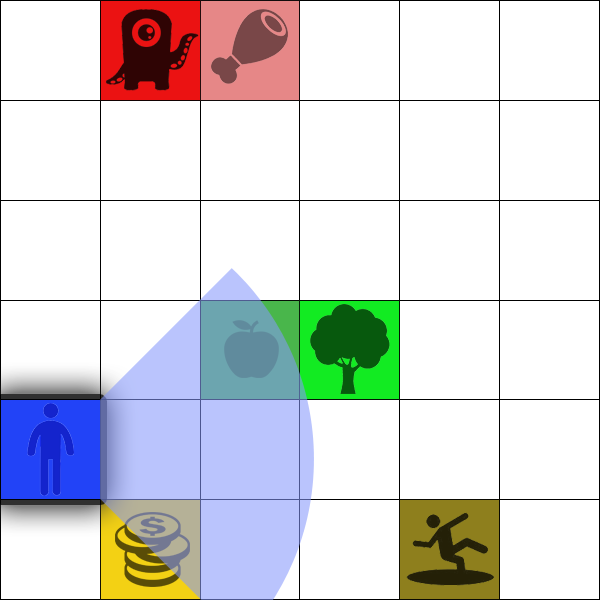
\includegraphics[width=0.65\textwidth]{map_agent.png}}%
         \only<3>{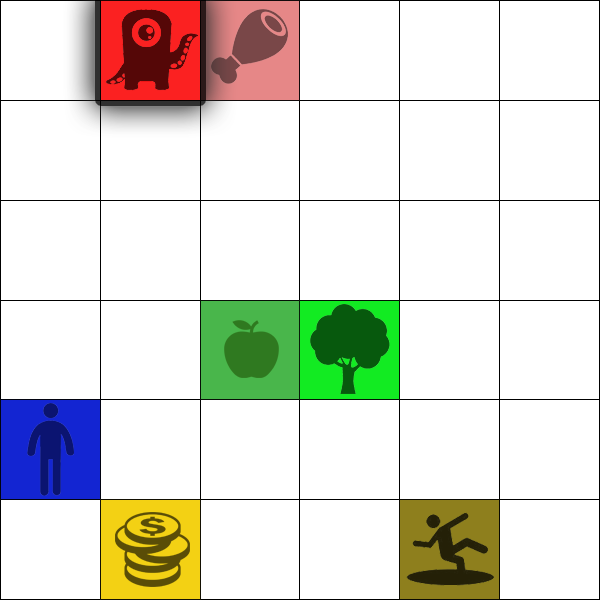
\includegraphics[width=0.65\textwidth]{map_wumpus.png}}%
         \only<4>{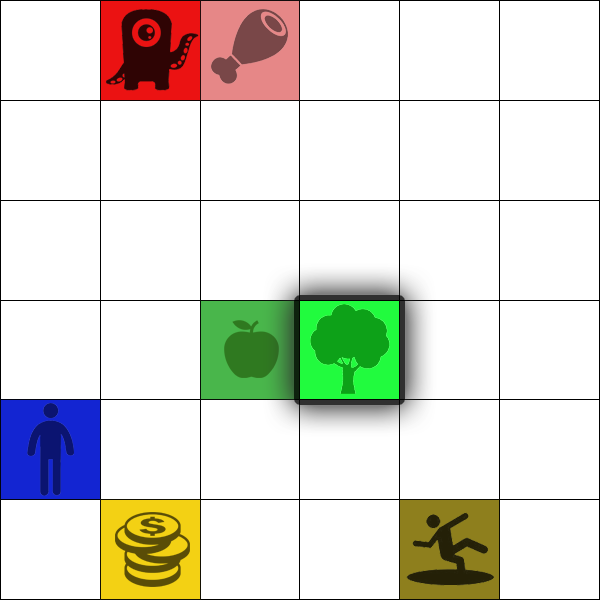
\includegraphics[width=0.65\textwidth]{map_plant.png}}%
         \only<5>{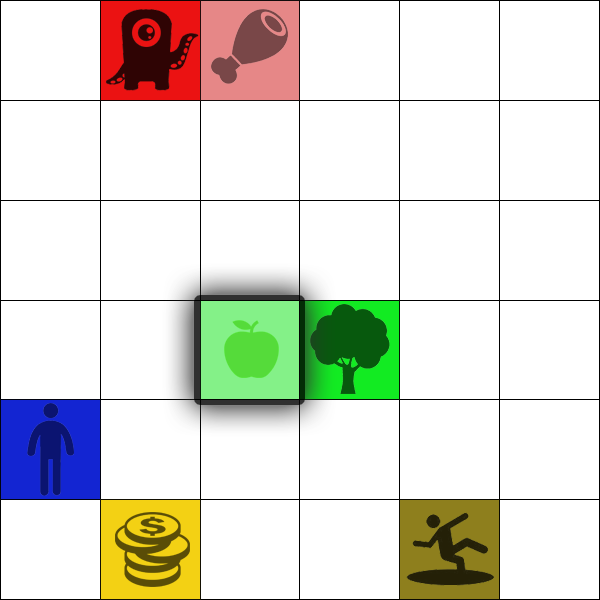
\includegraphics[width=0.65\textwidth]{map_fruit.png}}%
         \only<6>{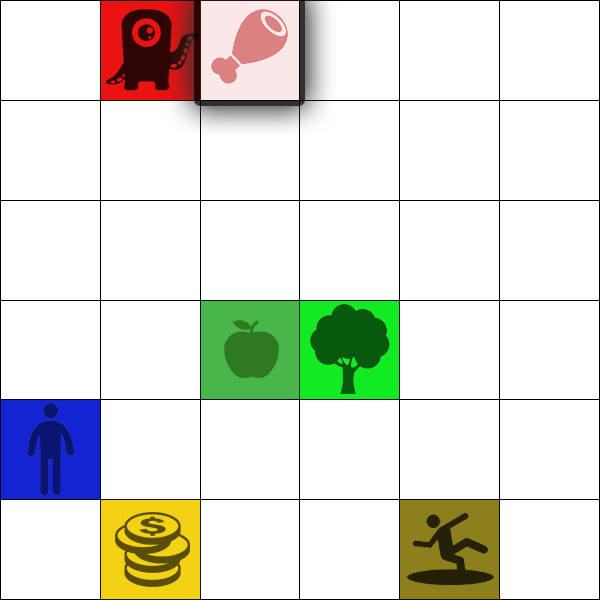
\includegraphics[width=0.65\textwidth]{map_meat.png}}%
         \only<7>{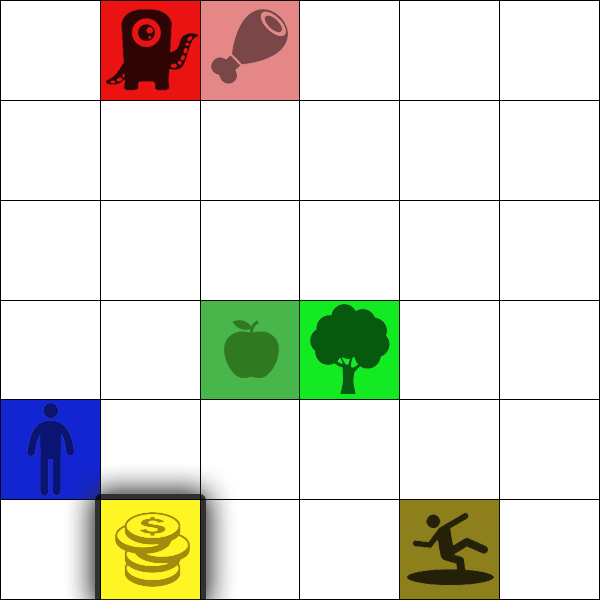
\includegraphics[width=0.65\textwidth]{map_gold.png}}%
         \only<8>{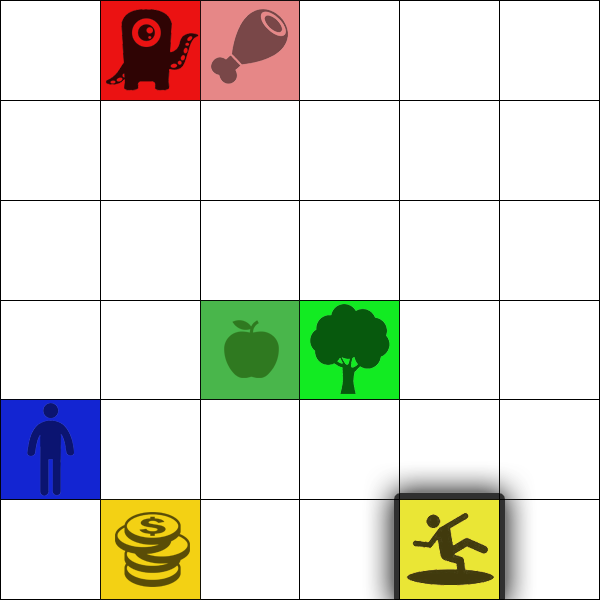
\includegraphics[width=0.65\textwidth]{map_pit.png}}%
      \end{center}
      %
      \begin{itemize}
         \setlength\itemsep{-1.25em}
         \item<1>Worlds are 2D grids.%
         \item<2>Agents see part of the world.%
         \item<3>Wumpuses seek and attack agents.%
         \item<4>Plants can be harvested.%
         \item<5>Fruit can be eaten.%
         \item<6>Meat can be eaten as well.%
         \item<7>Gold is just for ``trade''.%
         \item<8> Pits kill whatever falls into them.%
      \end{itemize}
   \end{frame}
   
   \begin{frame}{Architecture --- Agents}
      \begin{itemize}
         \item Based on evolutionary considerations, we designed 7 components.
         \vspace{2mm}
         \item Perception,
         \item Pre-social Behaviour Control (PSBC),
         \item Social Judgment System (SJS),
         \item Memory,
         \item Attention Control (AC),
         \item Decision Maker (DM), and
         \item Belief Generator (BG).
      \end{itemize}
      
      \tikzoverlay at (7.8cm,0.3cm) {
         \tikz node (label) at (0,0)[]{
            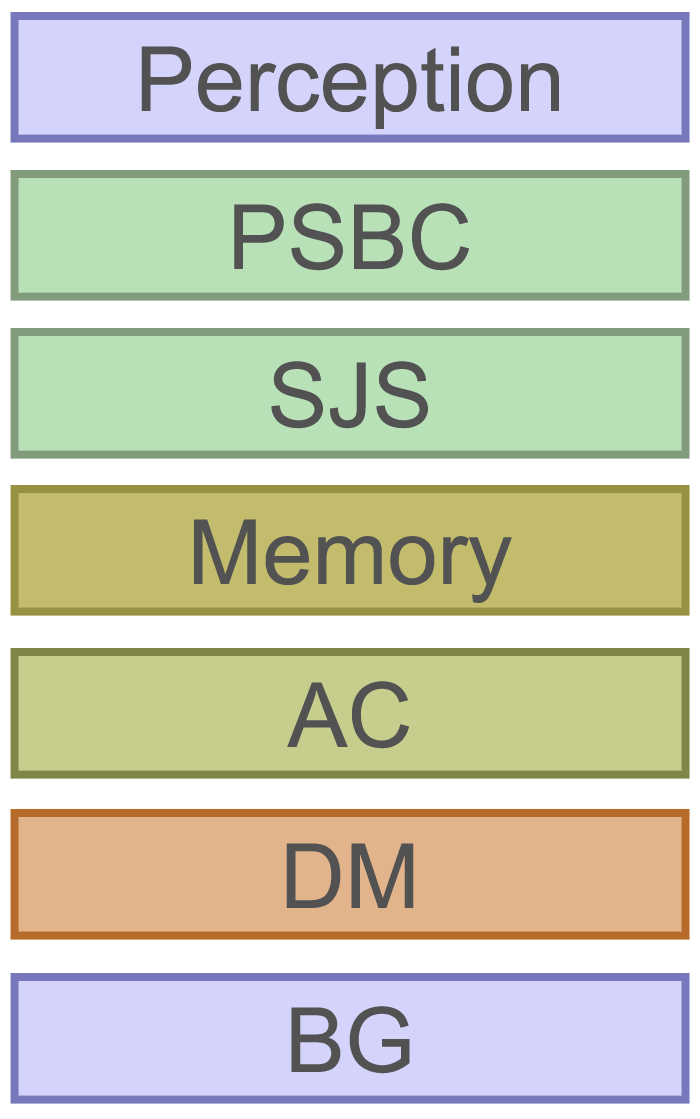
\includegraphics[width=3cm]{agent_components_intense.png}
         };
      };
   \end{frame}
   
   
   \begin{frame}{Architecture --- Agents}
      \begin{itemize}   
         \item Pre-Social Behaviour Control
         \pause
         \begin{itemize}
            \item The agent has four emotions:
            \begin{itemize}
               \item anger,
               \item fear,
               \item enthusiasm, and
               \item contentment.   
            \end{itemize}
         \end{itemize}
      \end{itemize}
   \end{frame}
   
   \begin{frame}{Architecture --- Agents}
      \begin{center}
         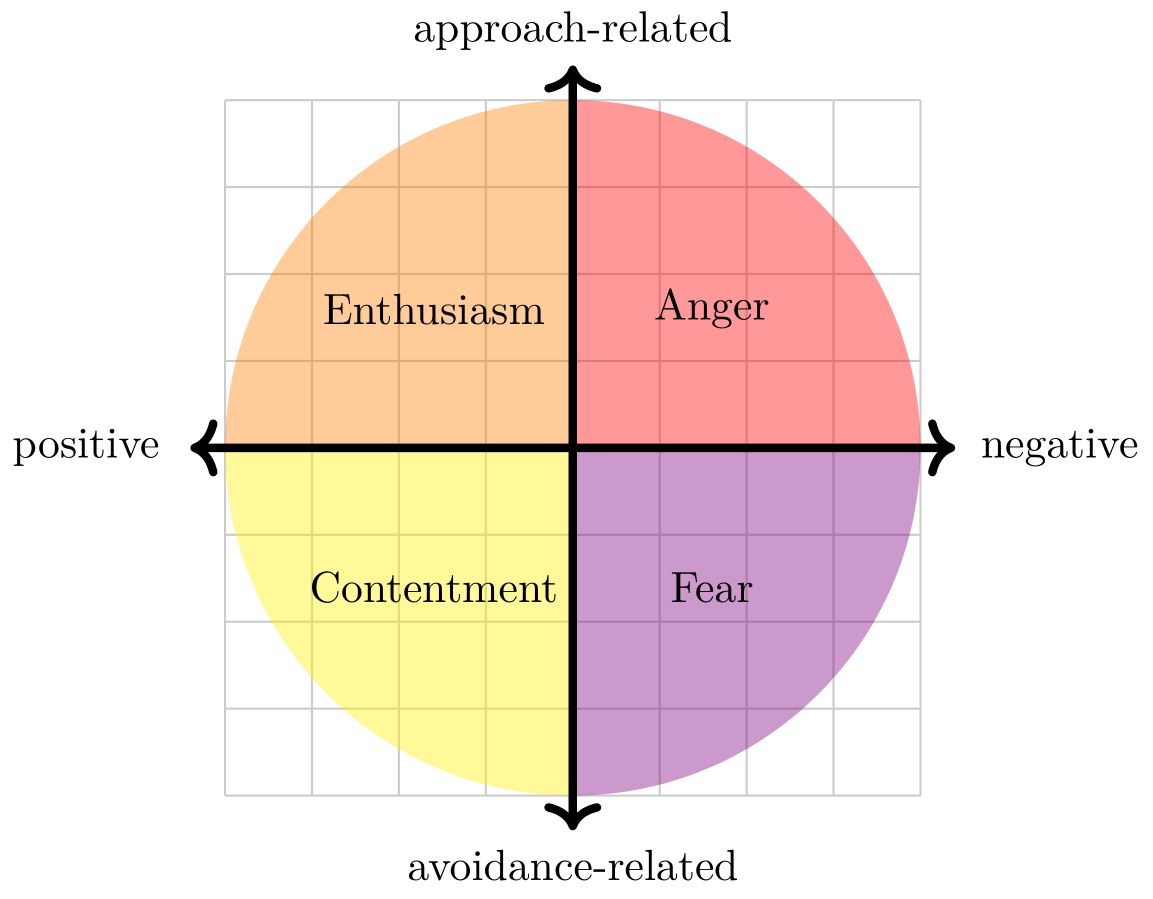
\includegraphics[width=0.8\textwidth]{../Thesis/Figs/PSBC.png}
      \end{center}
   \end{frame}
   
   \begin{frame}{Architecture --- Agents}
      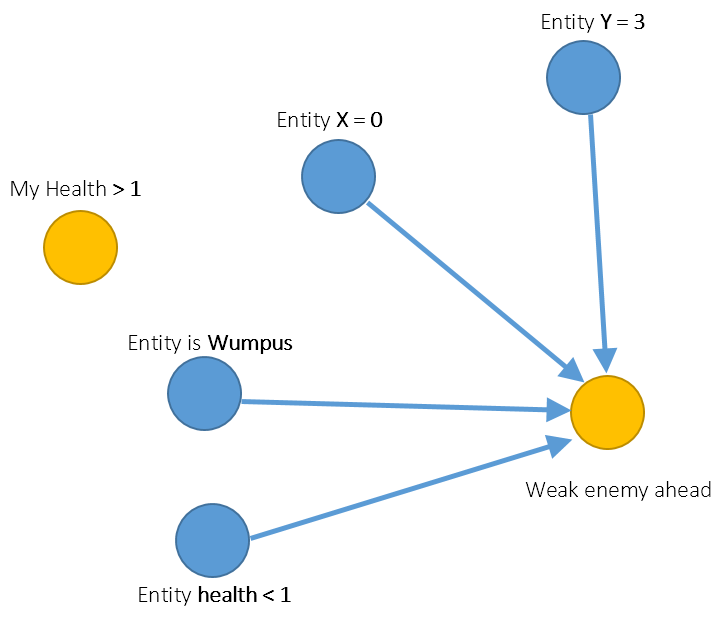
\includegraphics[width=0.8\textwidth]{anger_filter.png}
   \end{frame}
   
   \begin{frame}{Architecture --- Agents}
      \begin{itemize}
         \item {Social Judgment System}
         \begin{itemize}
            \item Other agents evoke
            \begin{itemize}
               \item sympathy,
               \item trust,
               \item respect.
            \end{itemize}
            \pause
            \item Every stranger has its own emotional levels.
            \item Agents can become friends (through positive interactions) or enemies.
         \end{itemize}
      \end{itemize}
      
      %      \tikzoverlay[text width=1.8cm] at (9.7cm,3.9cm) {
      %         \tikz node (label) at (0,0)[]{
      %            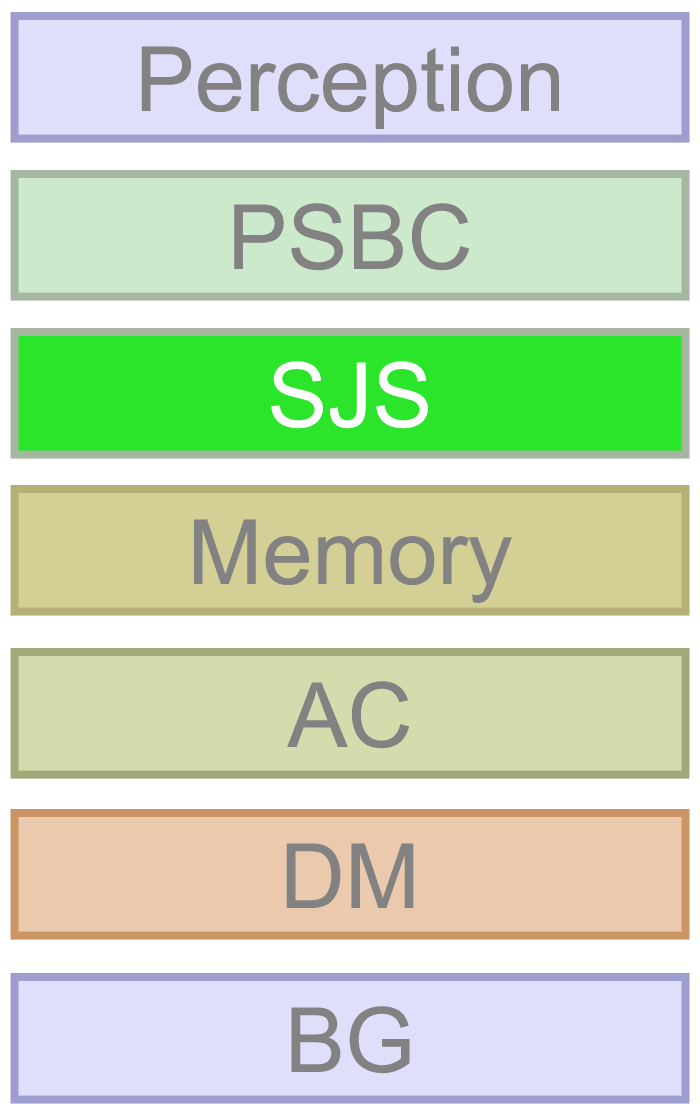
\includegraphics[width=1.8cm]{agent_components_sjs.png}
      %         };
      %      };
   \end{frame}
   
   \begin{frame}{Architecture --- Agents}
      \begin{itemize}
         \item Memory
         \begin{itemize}
            \item We store our perceptions for later recall.
            \item Memory can also store \cemph{imagined} worlds in a \cemph{tree structure}.
         \end{itemize}
         \pause
         \item Attention Control
         \begin{itemize}
            \item We assist the Decision Maker by selecting important targets.
            \item ``Important'' means ``evokes the strongest emotions''.
         \end{itemize}
      \end{itemize}
      
      %      \tikzoverlay[text width=2cm] at (9.5cm,3.3cm) {
      %         \tikz node (label) at (0,0)[]{
      %            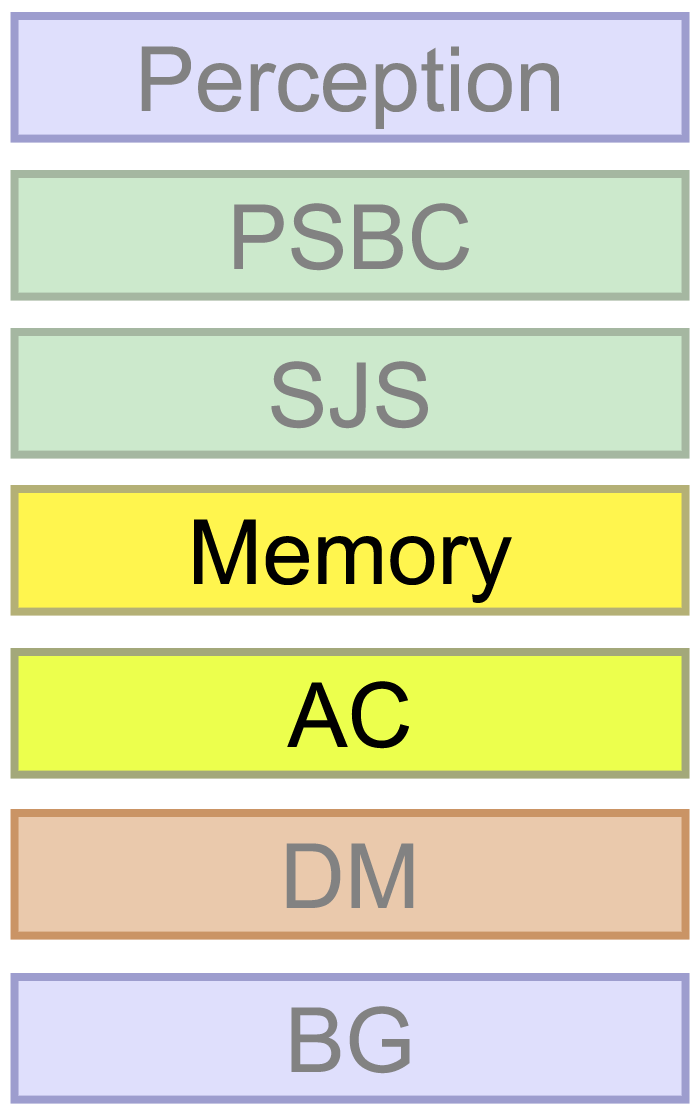
\includegraphics[width=2cm]{agent_components_memory_ac.png}
      %         };
      %      };
   \end{frame}
   
   \begin{frame}{Architecture --- Agents}
      \begin{itemize}
         \item Decision Maker
         \begin{itemize}
            \item Each emotion has some actions associated with it, e.g.,
            \begin{itemize}
               \item attacking is associated with anger,
               \item eating is associated with enthusiasm.
            \end{itemize}
            \pause
            \item The PSBC and the AC guide the planning:
            \begin{itemize}
               \item We select an action associated with our strongest emotion,
               \item and the cell(s) which have the most attention.
            \end{itemize}
            \pause
            \item If our emotion is strong enough, we take a \cemph{real} action,
            \item otherwise, we take a \cemph{hypothetical} one.
         \end{itemize}
      \end{itemize}
      
      %      \tikzoverlay[text width=1.8cm] at (9.7cm,3.9cm) {
      %         \tikz node (label) at (0,0)[]{
      %            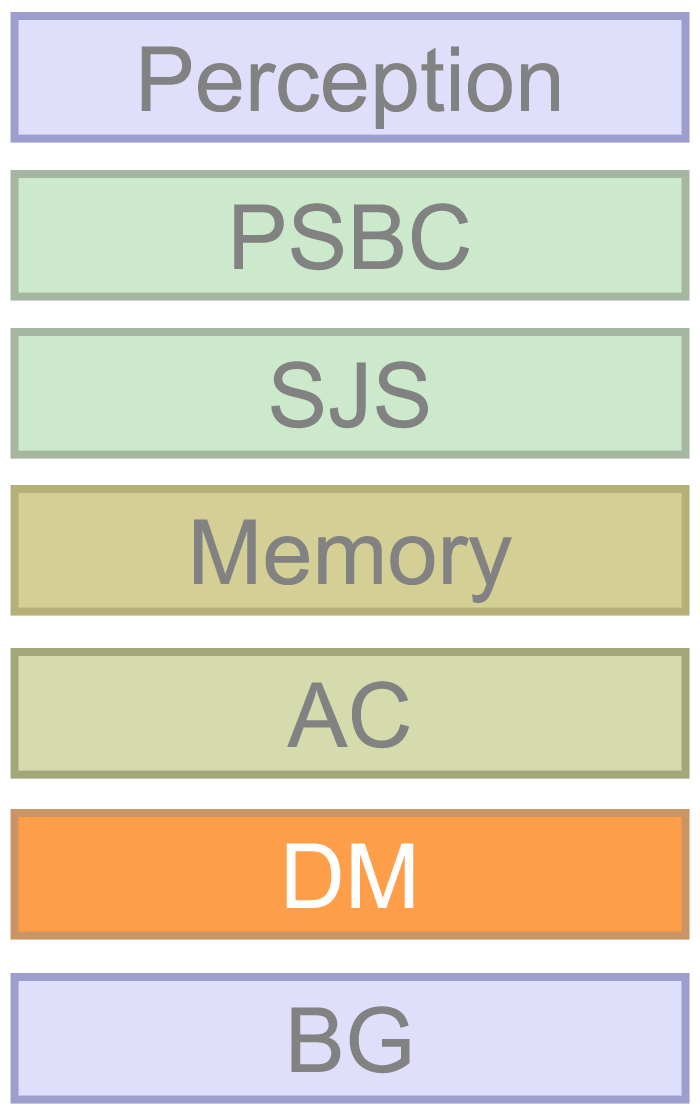
\includegraphics[width=1.8cm]{agent_components_dm.png}
      %         };
      %      };
   \end{frame}
   
   \begin{frame}{Architecture --- Agents}
      \begin{itemize}
         \item Belief Generator
         \begin{itemize}
            \item If the DM chose a \cemph{hypothetical} action, we simulate its consequences.
            \item We use the actual world simulator, but we construct the world from memory.
            \item The agent is then given \cemph{imagined perceptions}.
         \end{itemize}
      \end{itemize}
      
      %      \tikzoverlay[text width=1.8cm] at (9.7cm,3.9cm) {
      %         \tikz node (label) at (0,0)[]{
      %            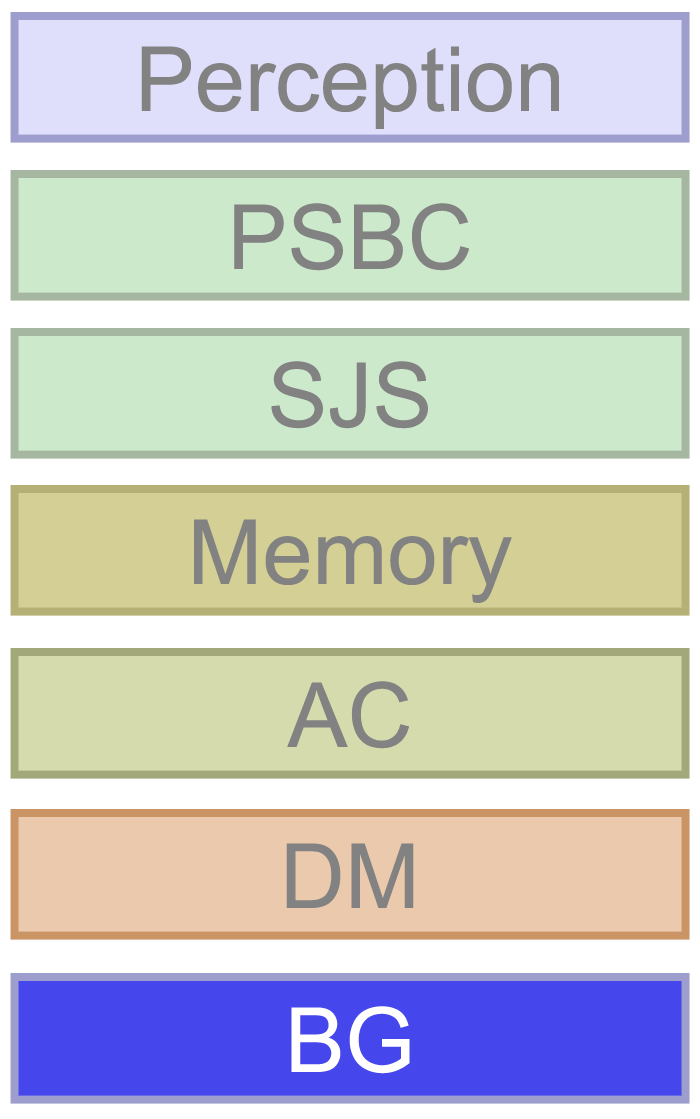
\includegraphics[width=1.8cm]{agent_components_bg.png}
      %         };
      %      };
   \end{frame}
   
   \begin{frame}{Architecture --- Agents}
      \begin{itemize}
         \item {How does this all fit together?}
      \end{itemize}
      
      \begin{center}
         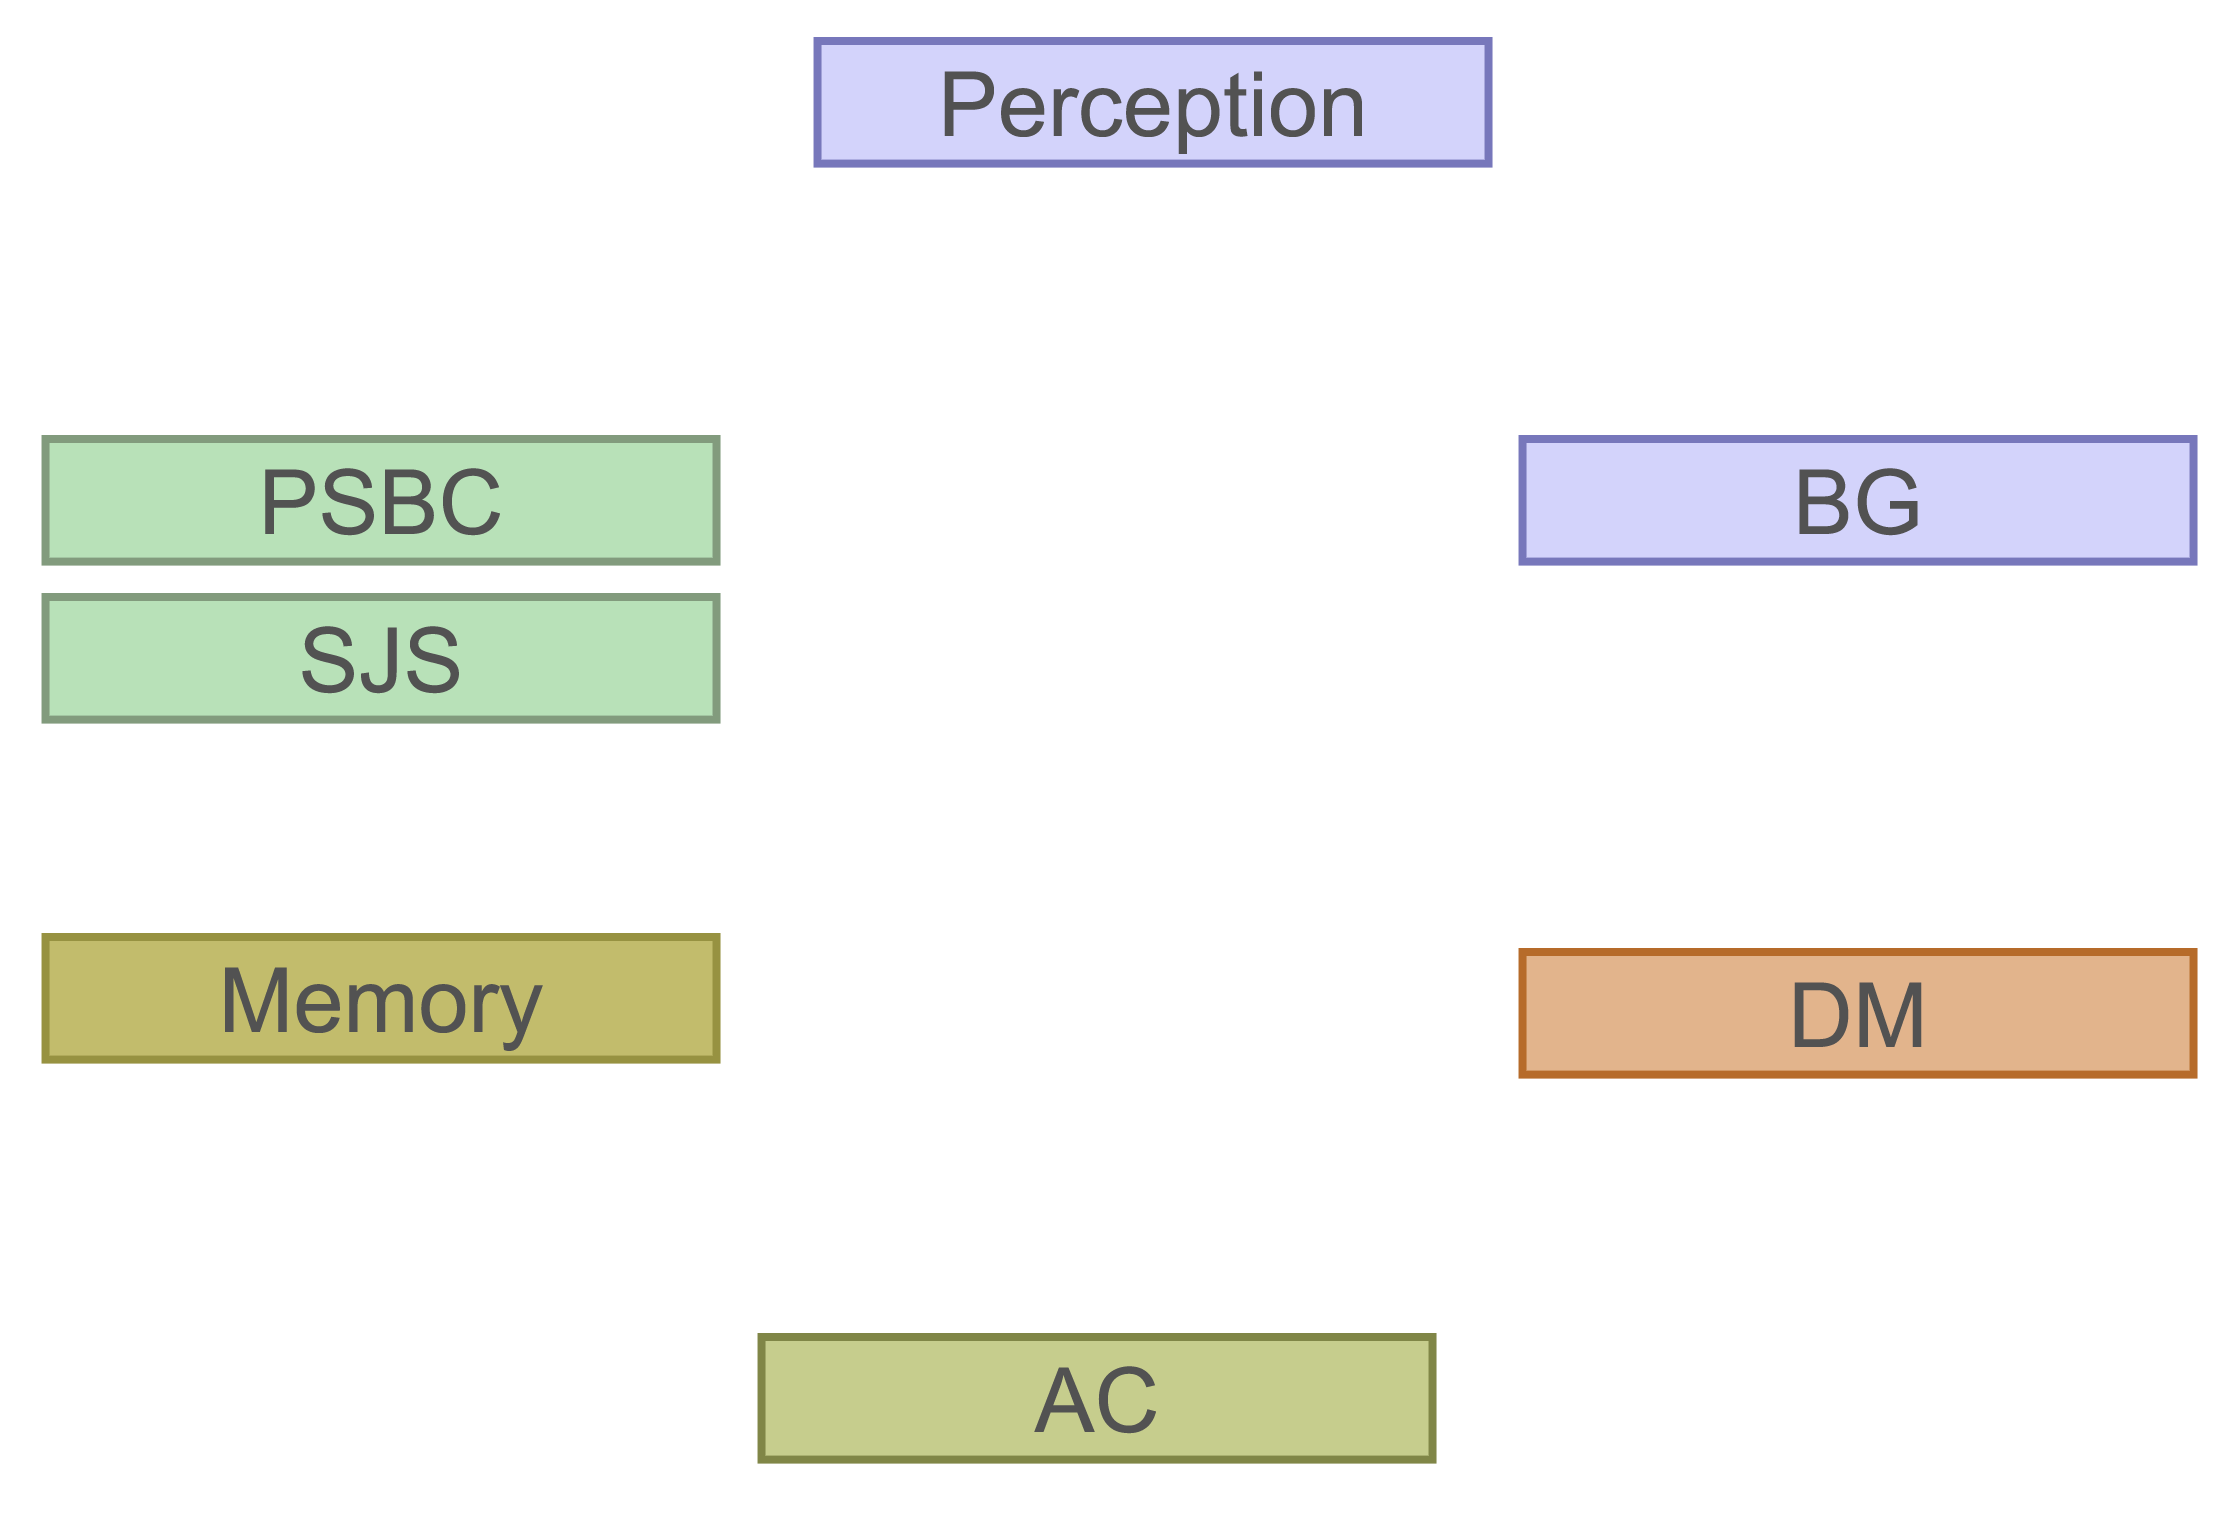
\includegraphics[width=0.8\textwidth]{plan_0.png}
      \end{center}
      
      ~
   \end{frame}
   
   \begin{frame}{Architecture --- Agents}
      \begin{itemize}
         \item {How does this all fit together?}
      \end{itemize}
      
      \begin{center}
         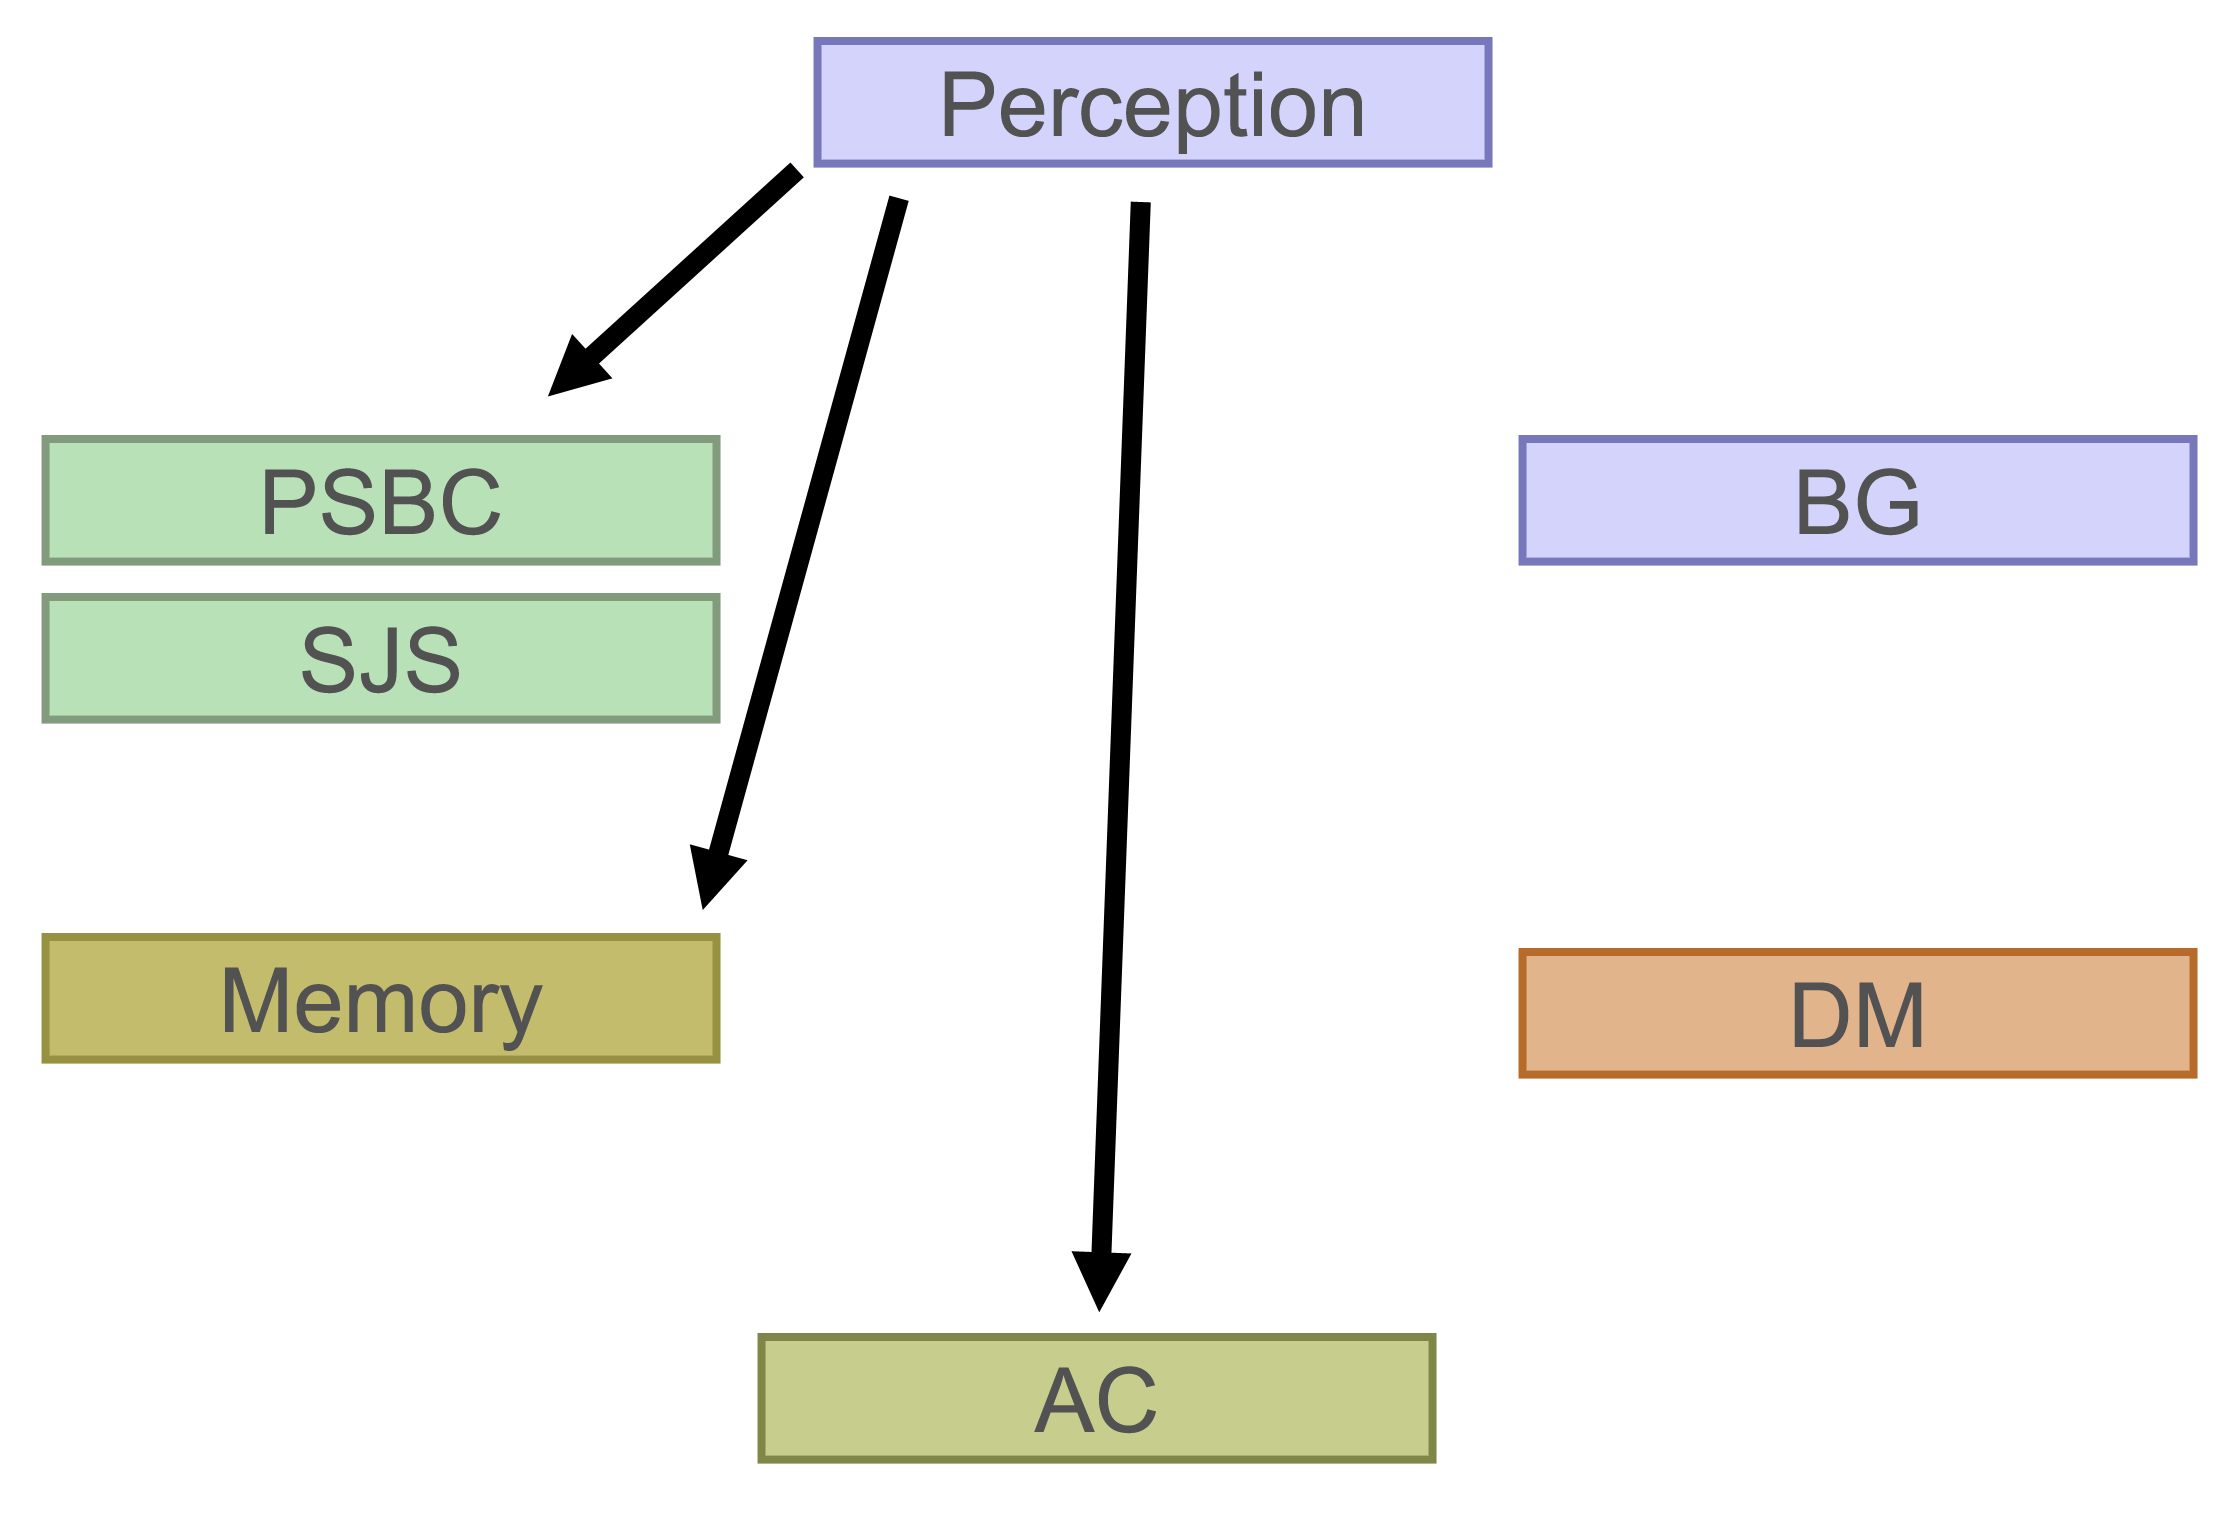
\includegraphics[width=0.8\textwidth]{plan_1.png}
      \end{center}
      
      \cemph{Perception} distributes its messages.
   \end{frame}
   
   \begin{frame}{Architecture --- Agents}
      \begin{itemize}
         \item {How does this all fit together?}
      \end{itemize}
      
      \begin{center}
         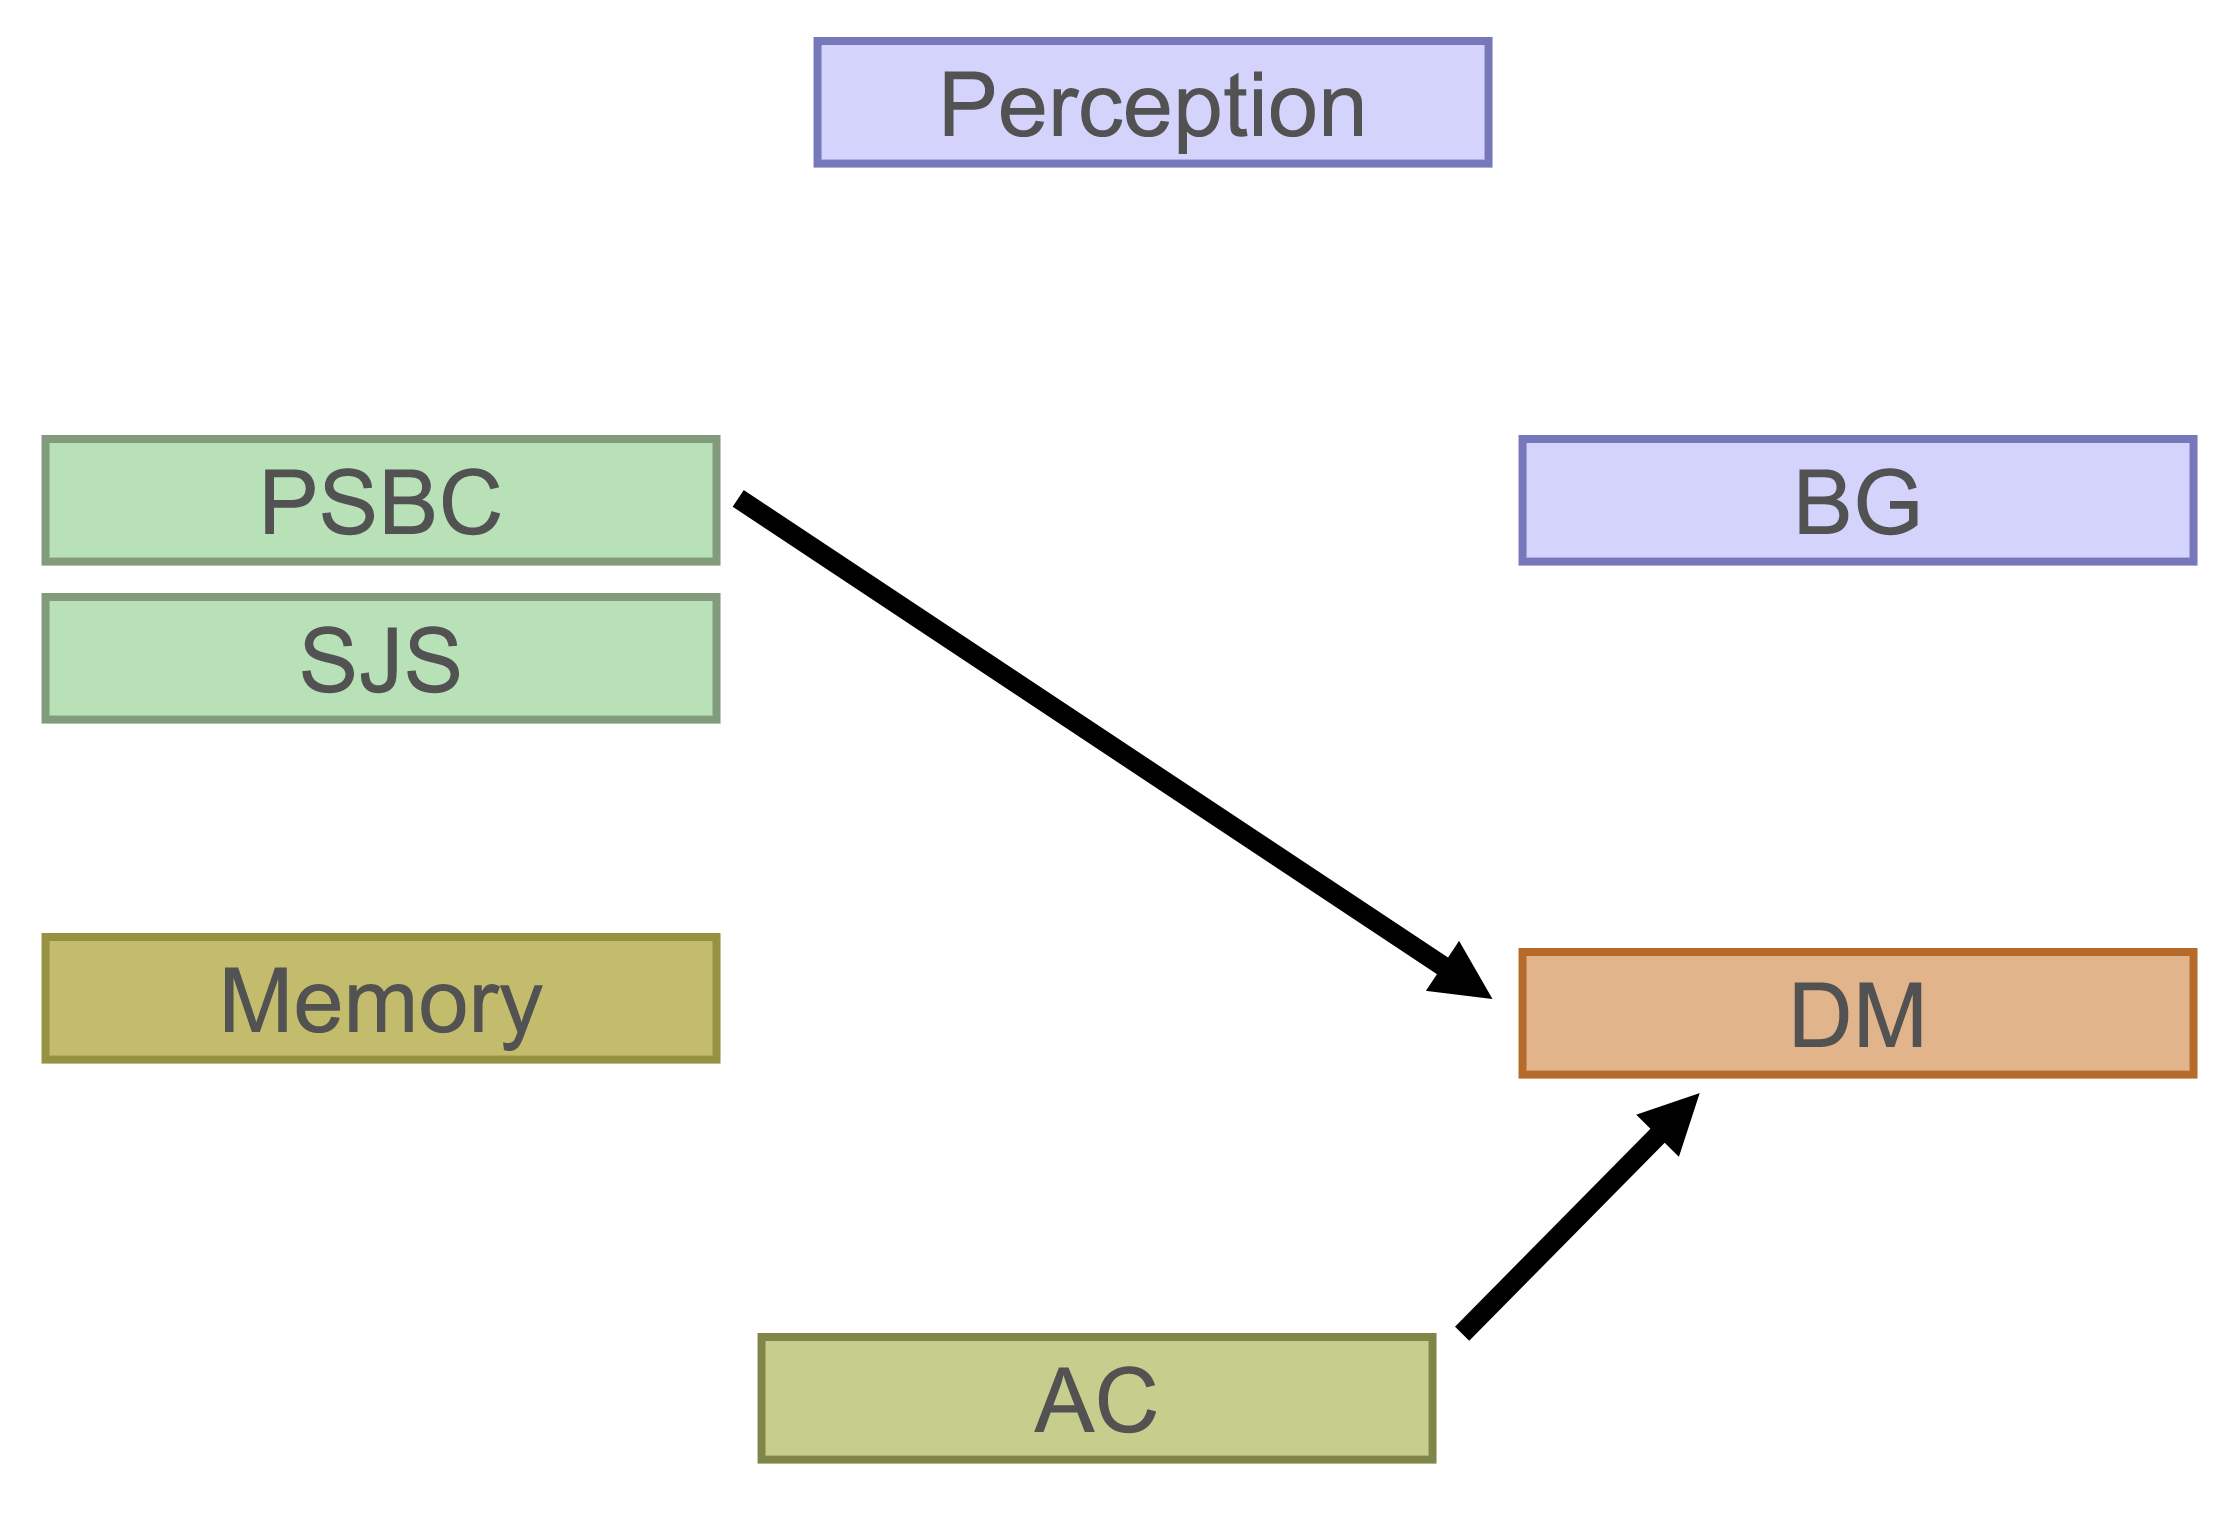
\includegraphics[width=0.8\textwidth]{plan_2.png}
      \end{center}
      
      The \cemph{Decision Maker} is informed about the affective reactions.
   \end{frame}
   
   \begin{frame}{Architecture --- Agents}
      \begin{itemize}
         \item {How does this all fit together?}
      \end{itemize}
      
      \begin{center}
         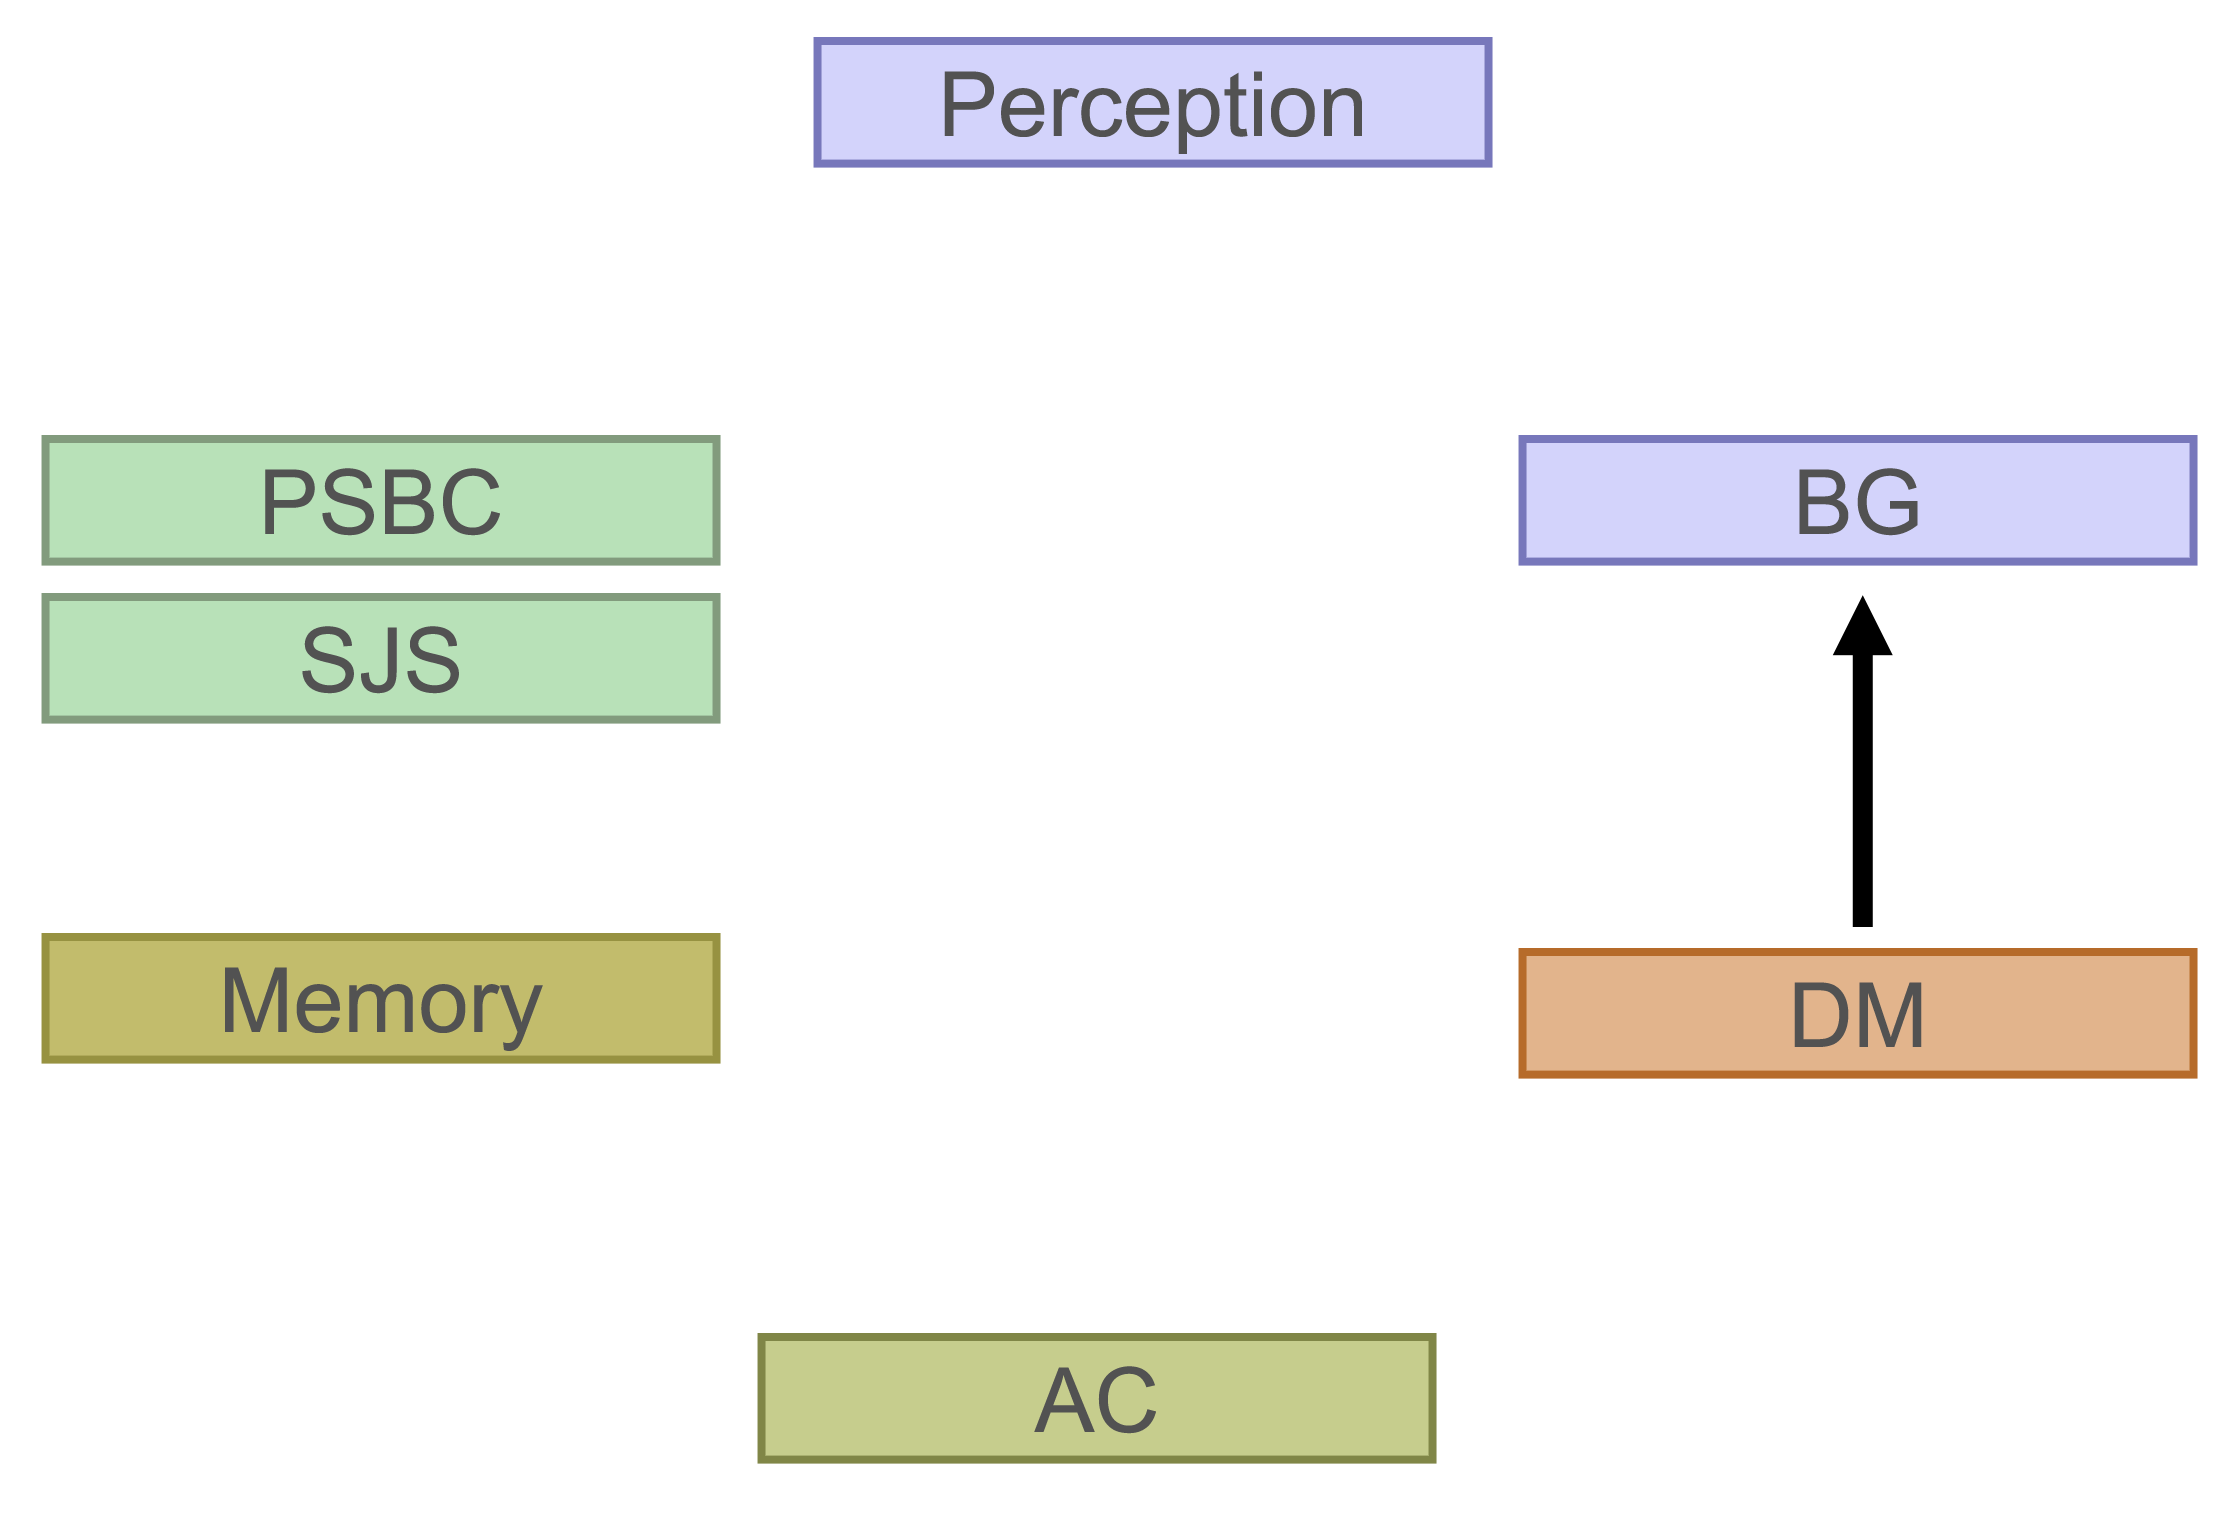
\includegraphics[width=0.8\textwidth]{plan_3.png}
      \end{center}
      
      Option 1: The \cemph{Belief Generator} simulates the consequences.
   \end{frame}
   
   \begin{frame}{Architecture --- Agents}
      \begin{itemize}
         \item {How does this all fit together?}
      \end{itemize}
      
      \begin{center}
         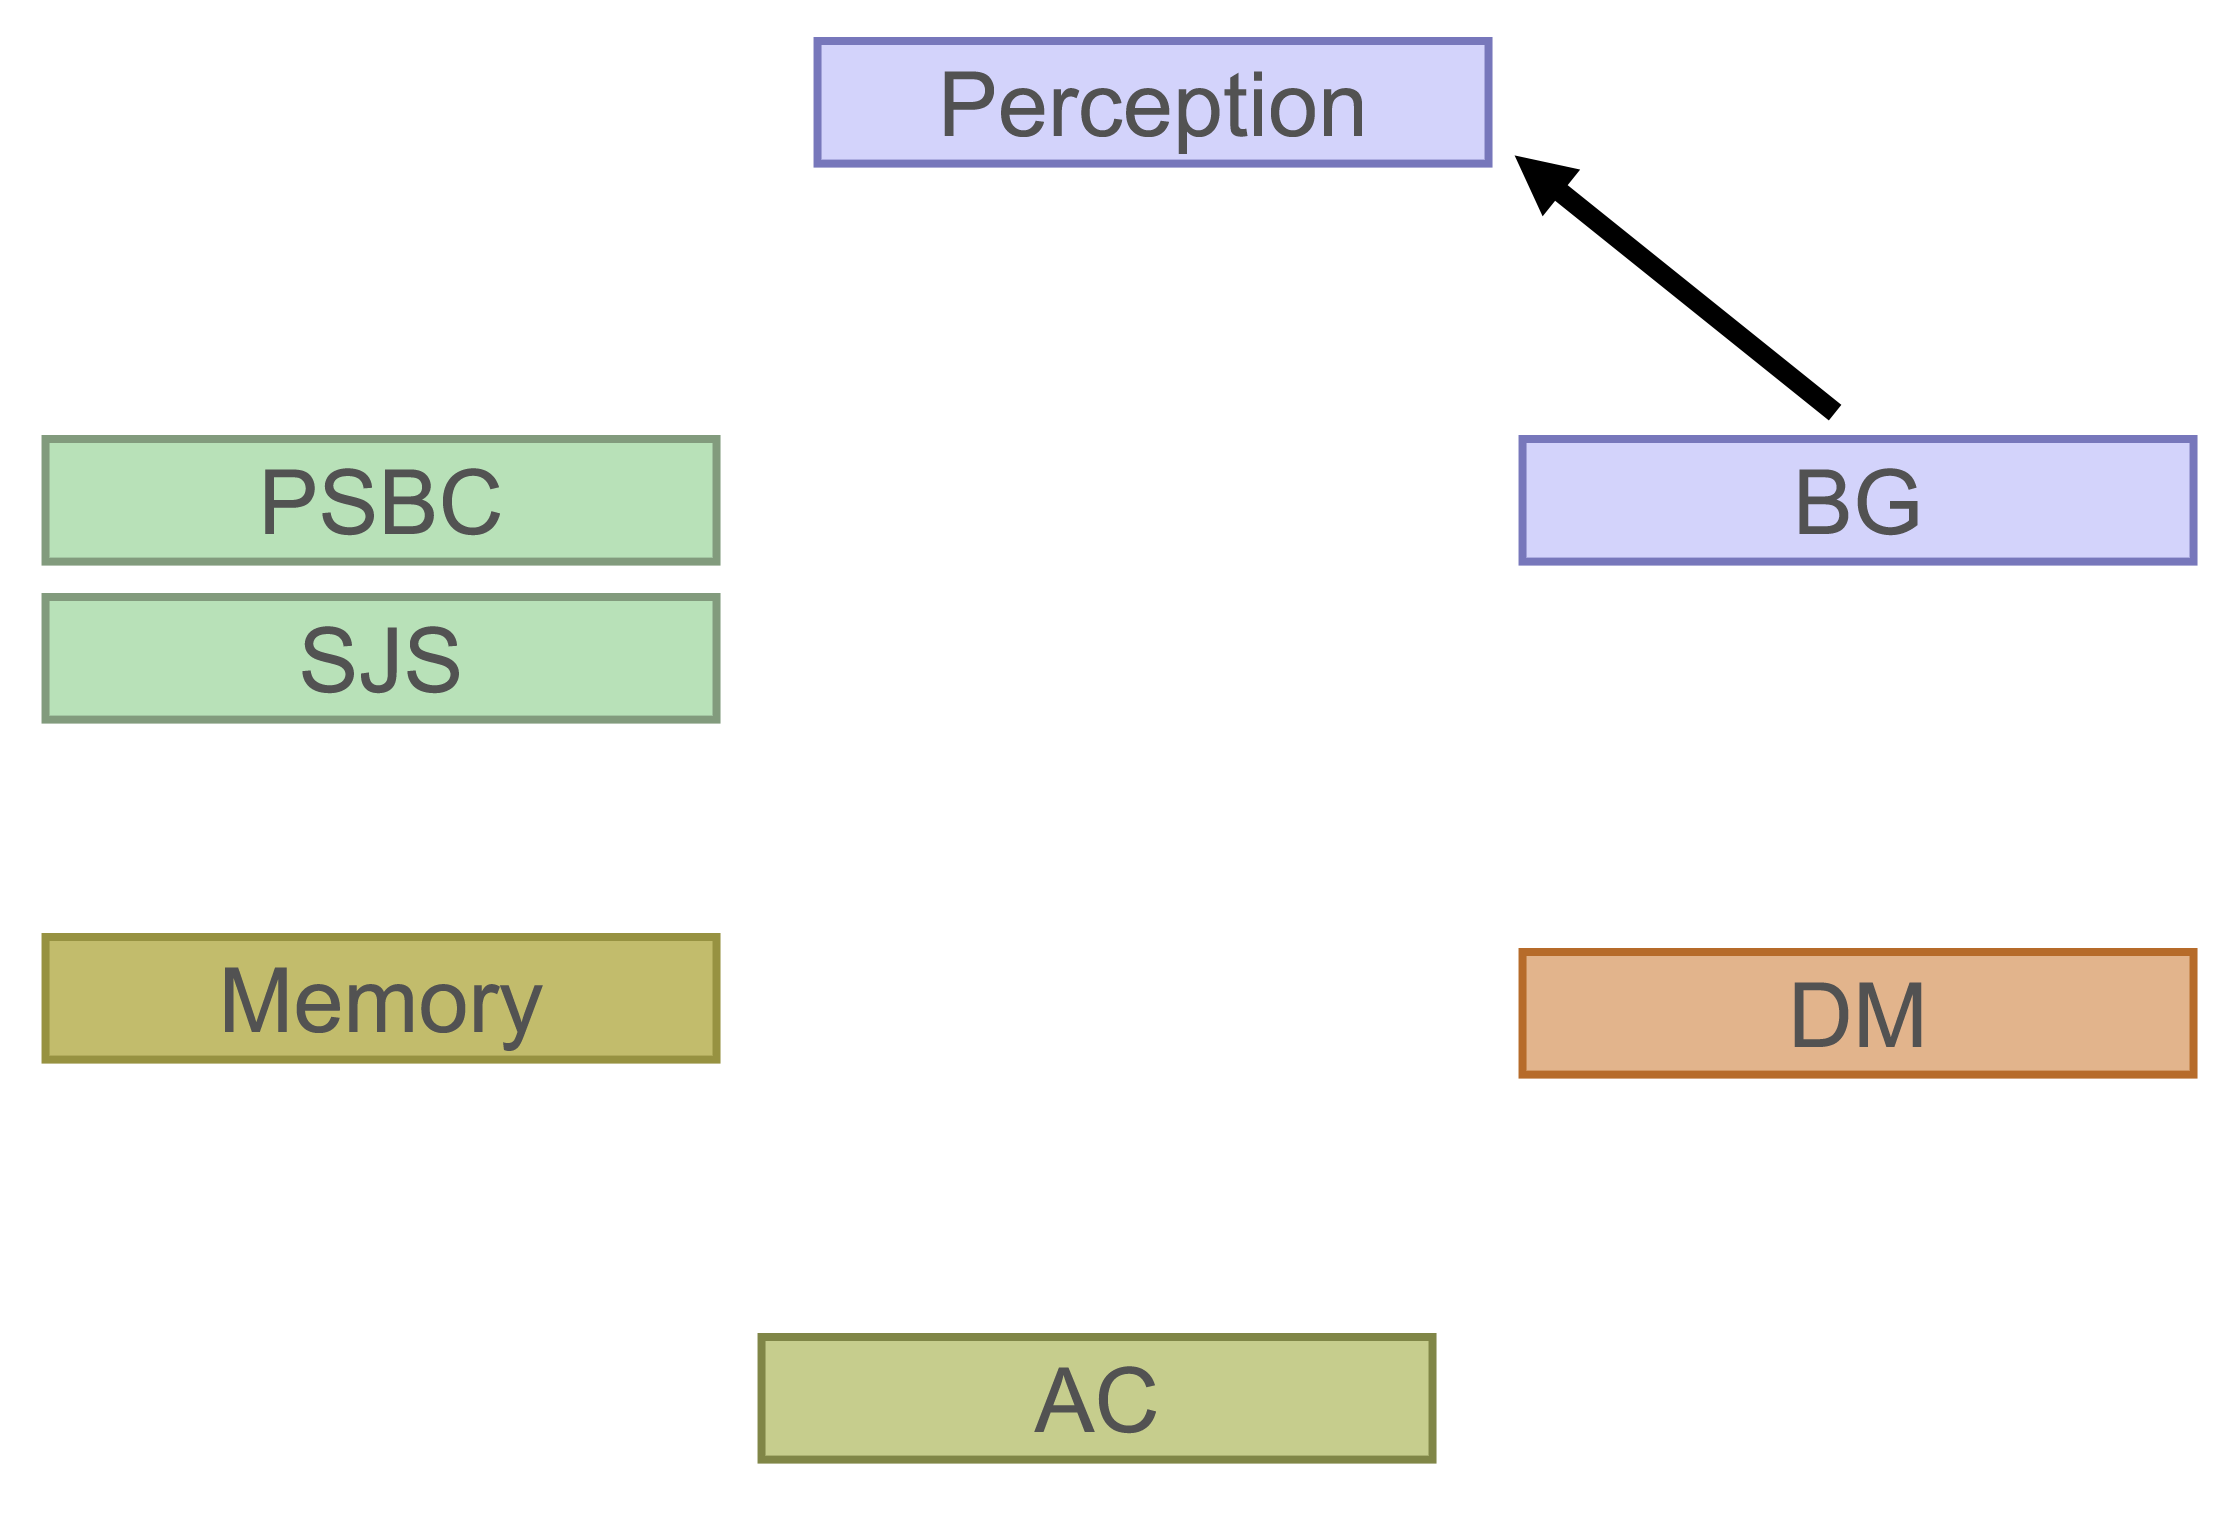
\includegraphics[width=0.8\textwidth]{plan_4.png}
      \end{center}
      
      The loop begins anew, but with \cemph{imagined} perceptions.
   \end{frame}
   
   \begin{frame}{Architecture --- Agents}
      \begin{itemize}
         \item {How does this all fit together?}
      \end{itemize}
      
      \begin{center}
         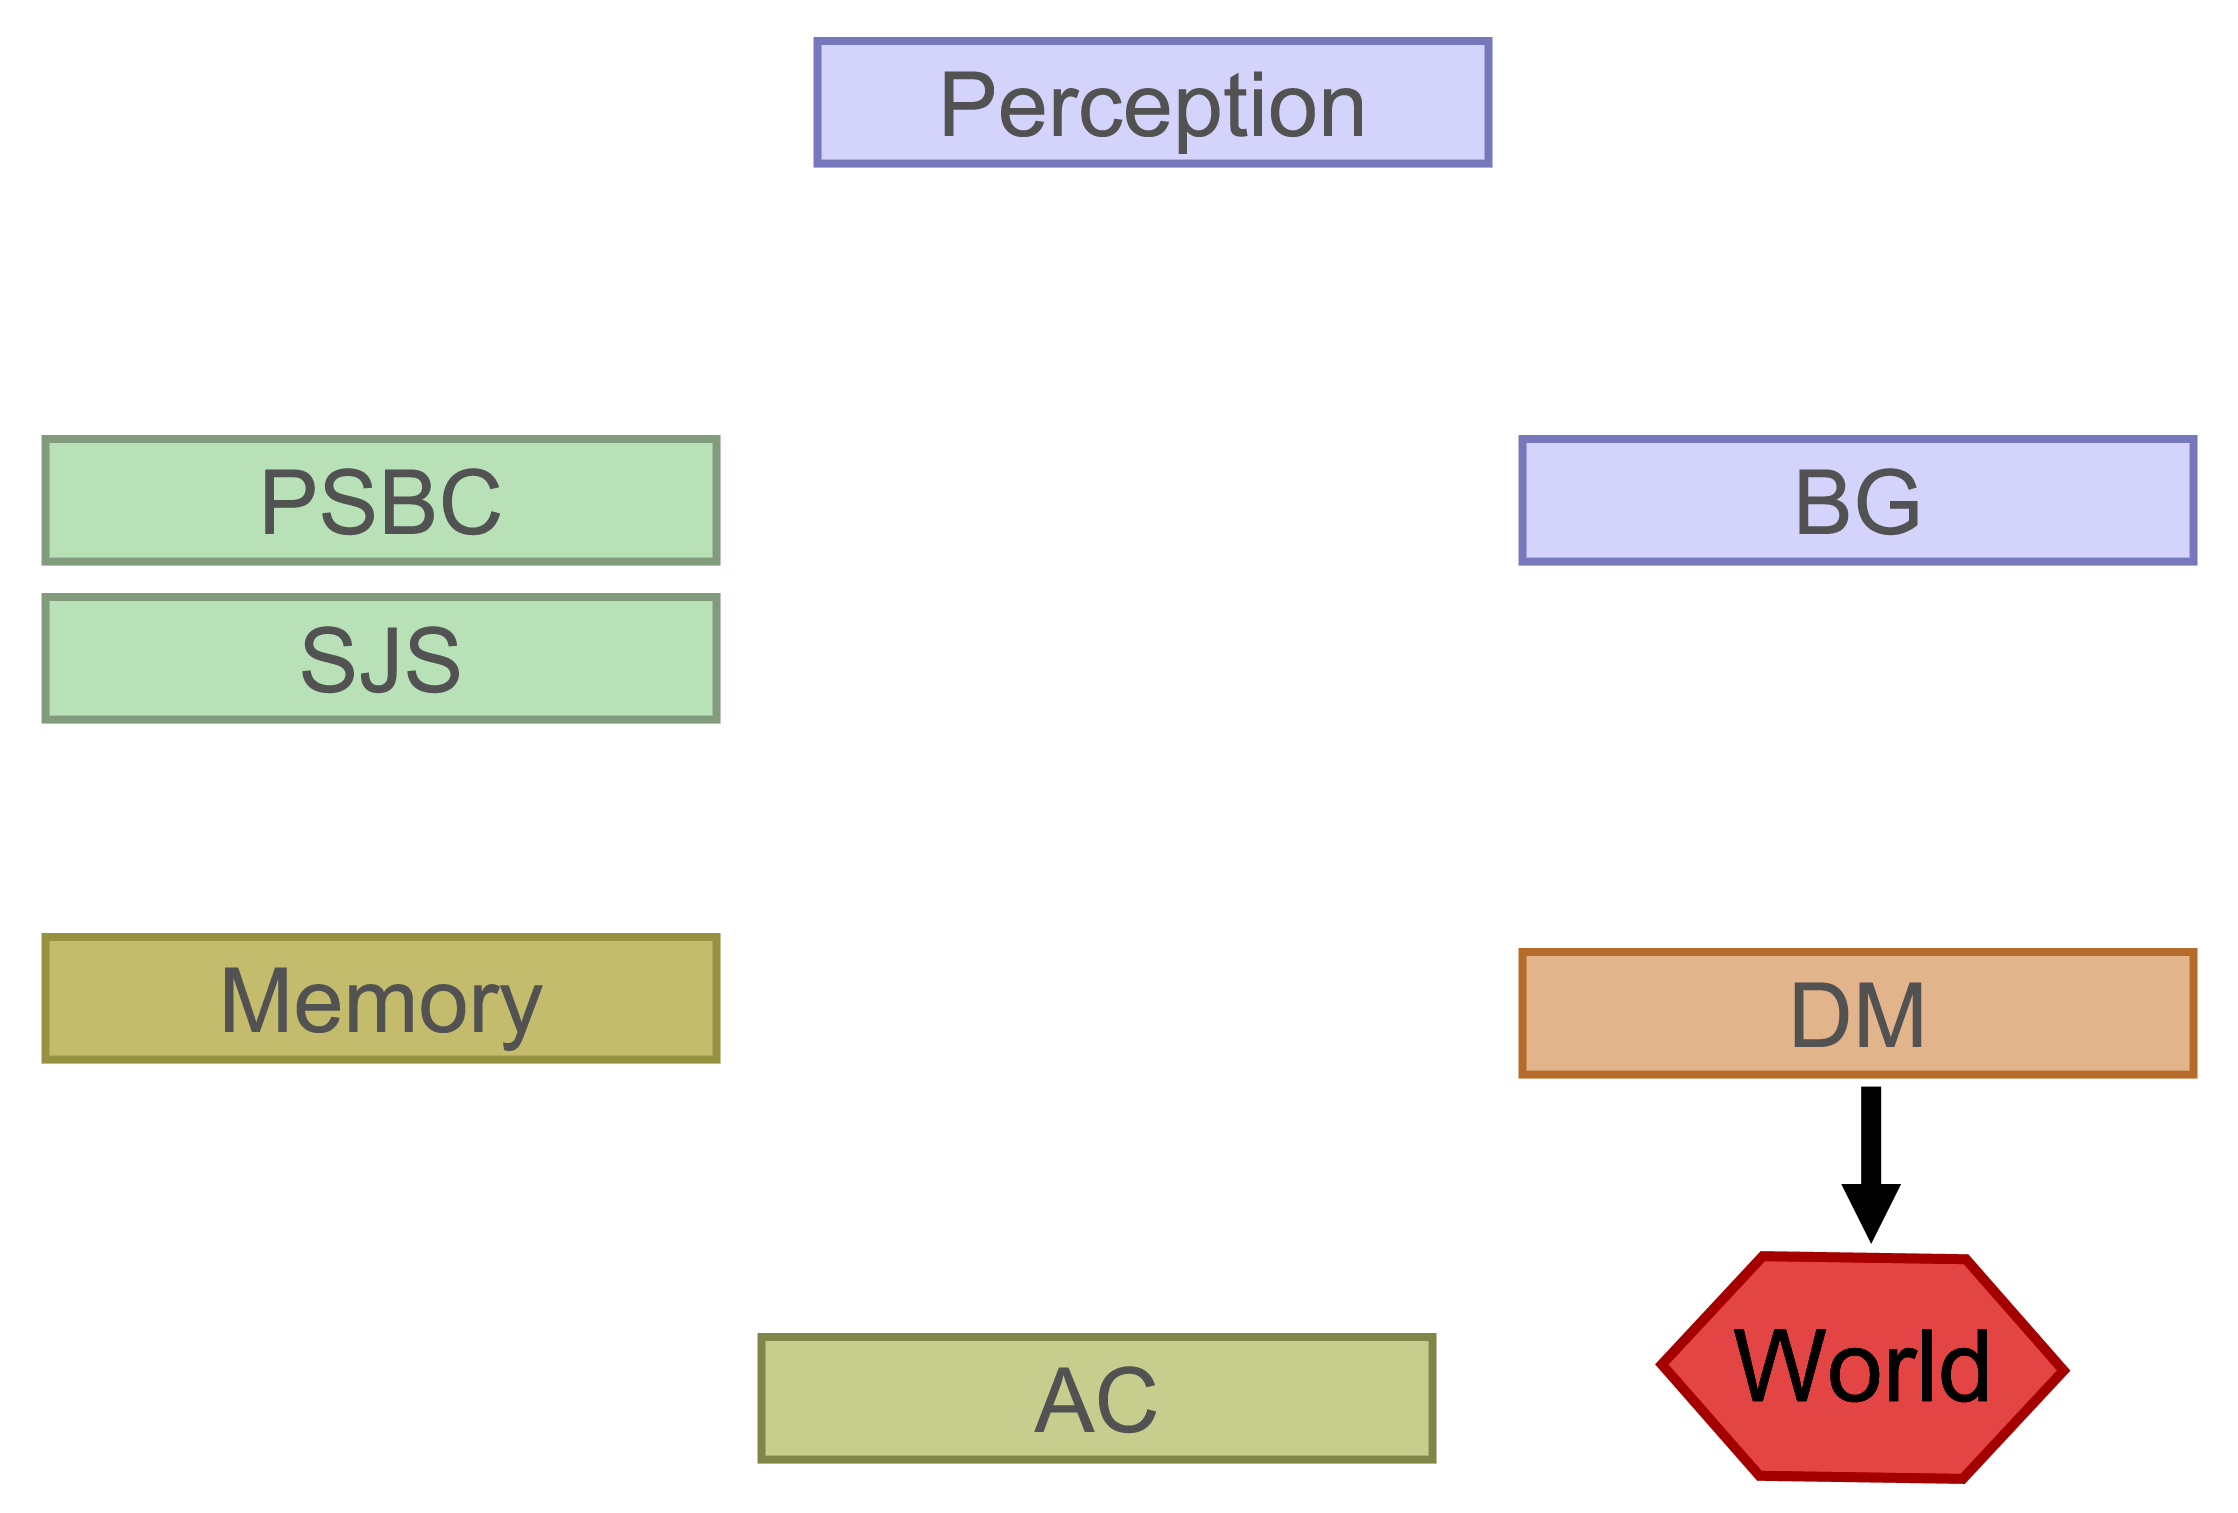
\includegraphics[width=0.8\textwidth]{plan_5.png}
      \end{center}
      
      Option 2: The \cemph{Decision Maker} chooses a real action.
   \end{frame}
   
   \begin{frame}{Architecture --- Agents}
      \begin{itemize}
         \item To simplify it: DM and BG are in a loop.
      \end{itemize}
      
      \begin{center}
         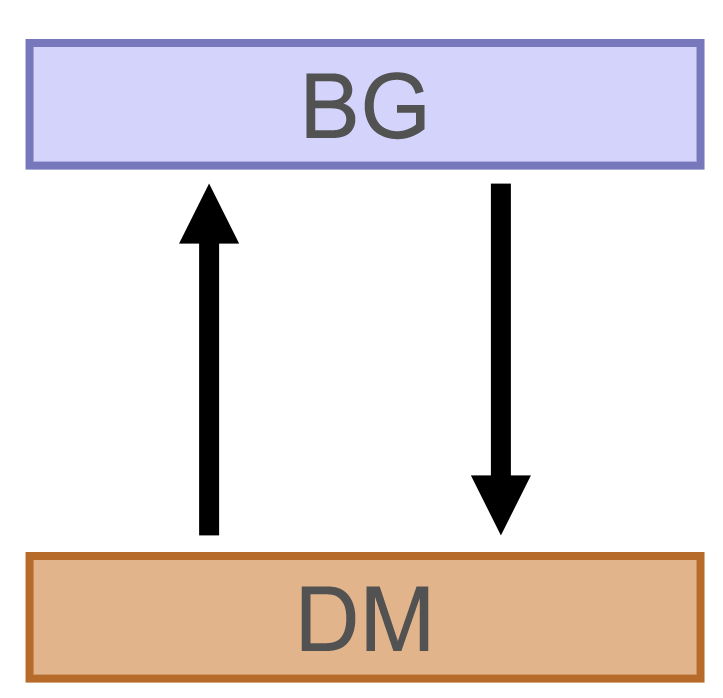
\includegraphics[width=0.3\textwidth]{bg_dm_loop.png}
      \end{center}
      
      \begin{enumerate}
         \item We choose a \cemph{hypothetical} action,
         \item Then we simulate its consequences.
      \end{enumerate}
      
      \begin{itemize}
         \item We repeat this until the DM deems the outcome satisfactory and chooses a \cemph{real} action.
      \end{itemize}
   \end{frame}
   
   \begin{frame}{Architecture --- Agents}
      \begin{itemize}
         \item An example plan.
         \item Our agent is hungry, but has no food.
         \item There is a plant some distance away.
      \end{itemize}
      
      \medskip
      
      \begin{tabular}{c c}
         \hspace{1cm}\parbox{0.4\textwidth}{\vspace{-3cm}
            Plan:\\
            Move North.\\
            Move North.\\
            Harvest plant.\\
            Eat fruit.\\}
         
         & 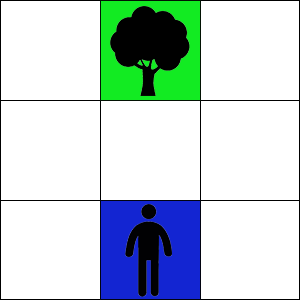
\includegraphics[width=0.3\textwidth]{hungry_agent.png}
      \end{tabular}
   \end{frame}
   
   \section{Evaluation}
   
   \begin{frame}{Evaluation}
      \begin{itemize}
         \item We created 32 populations with different personalities
         \item and simulated 50 rounds with each population.
         \item We combined weak/strong anger, fear, enthusiasm, contentment, as well as hostility.
         \begin{itemize}
            \item Example personality: $\personality{S}{W}{S}{W}{S}$\\
            meaning ``strong anger, weak fear, strong enthusiasm, weak contentment, strong hostility''.
         \end{itemize}
         \item Throughout the simulation, we collected data: the number of
         \begin{itemize}
            \item gifts given,
            \item surviving Wumpuses,
            \item surviving agents,
            \item plants harvested, etc.
         \end{itemize}
      \end{itemize}
   \end{frame}
   
   \begin{frame}{Results}
      \begin{itemize}
         \item Initially, there were 30 agents.
         \item We averaged survival over all personalities with weak anger, strong anger, weak enthusiasm, etc.
      \end{itemize}
      
      \begin{table}
         \centering
         \only<1>{%
            \begin{tabular}{ l | c | c | c}
               \emph{Personality fragment} & \emph{weak} & \emph{ strong} & $\Delta$ \\
               \hline
               Anger & 80.8\% & 74.4\% & -6.4\\
               Fear & 74.8\% & 80.4\% & 5.6\\
               Enthusiasm & 75.8\% & 79.4\% & 3.6\\
               Contentment & 76.9\% & 78.3\% & 1.4\\
               Hostility & 76.4\% & 78.8\% & 2.4\\
               \hline
            \end{tabular}}
            \only<2>{%
               \begin{tabular}{ l | c | c | c}
                  \emph{Personality fragment} & \emph{weak} & \emph{ strong} & $\Delta$ \\
                  \hline
                  \rowcolor{LightGreen}Anger&\cellcolor{IntenseGreen}80.8\%&74.4\% & -6.4\\
                  Fear & 74.8\% & 80.4\% & 5.6\\
                  Enthusiasm & 75.8\% & 79.4\% & 3.6\\
                  Contentment & 76.9\% & 78.3\% & 1.4\\
                  Hostility & 76.4\% & 78.8\% & 2.4\\
                  \hline
               \end{tabular}}
               \only<3>{%
                  \begin{tabular}{ l | c | c | c}
                     \emph{Personality fragment} & \emph{weak} & \emph{ strong} & $\Delta$  \\
                     \hline
                     \rowcolor{LightGreen}Anger&\cellcolor{IntenseGreen}80.8\%&74.4\% & -6.4\\
                     \rowcolor{LightYellow}Fear&74.8\%&\cellcolor{IntenseYellow}80.4\% & 5.6\\
                     Enthusiasm & 75.8\% & 79.4\% & 3.6\\
                     Contentment & 76.9\% & 78.3\% & 1.4\\
                     Hostility & 76.4\% & 78.8\% & 2.4\\
                     \hline
                  \end{tabular}}
                  \caption{Average number of surviving agents, by personality fragment.}
                  \label{tab:numAgentsAvg}
               \end{table}
               
               \begin{itemize}
                  \item<3-> Weak anger and strong fear are useful!
               \end{itemize}
            \end{frame}
            
            \begin{frame}{Results}
               \begin{itemize}
                  \item There were some surprising results.
                  \item Agents were able to give gifts (meat, fruit, gold) to others.
               \end{itemize}
               
               \begin{table}
                  \centering
                  \begin{tabular}{ l | c }
                     \emph{Personality} & \emph{Meat gifts} \\
                     \hline
                     
                     $\personality{S}{W}{W}{W}{S}$ & 0\\
                     $\personality{W}{W}{W}{W}{S}$ & 0\\
                     $\personality{S}{W}{W}{S}{W}$ & 1\\
                     \multicolumn{2}{c}{$\dots$}\\
                     $\personality{S}{W}{S}{W}{W}$ & 19\\
                     $\personality{S}{W}{S}{W}{S}$ & 19\\
                     \hline
                  \end{tabular}
                  \caption{Number of meat items given as gifts after 50 rounds.}
                  \label{tab:numWumpuses}
               \end{table}
               \begin{itemize}
                  \item $\personality{S}{W}{S}{W}{S}$ means ``strong anger, weak fear, strong enthusiasm, weak contentment, strong hostility''.
                  \item Agents with strong anger and weak fear killed everything and shared the meat among themselves.
               \end{itemize}
            \end{frame}
            
            \section{Conclusion}
            
            \begin{frame}{Conclusion}
               \begin{itemize}
                  \item We designed an agent architecture based on evolutionary considerations.
                  \pause
                  \item Our aim was to approximate real organisms.
                  \pause
                  \item Agents were put into a moderately complex game world
                  \pause
                  \item and performed reasonably well.
                  \pause
                  \item Personalities differentiated themselves in interesting ways.
               \end{itemize}
            \end{frame}
            
            \begin{frame}[plain, c]
               \begin{center}
                  \huge Thank you for your attention!
               \end{center}
            \end{frame}
\end{document}
